\chapter{Additional jet distributions in the signal regions}
    \label{app:SRkimenaticDistr}

This appendix collects the most relevant distributions for jets in the final state, in the signal regions M1 to M6.
The distributions for the leading jet and $\met$ $\phi$, the $\Delta\Phi$ between the leading jet and the $\met$, the leading jet charged fraction, the second leading jet $\pt$, the jet multiplicity, and the second leading jet $\eta$ and $\phi$ are shown.

\begin{figure}[!ht]
  \begin{center}
    \mbox{
      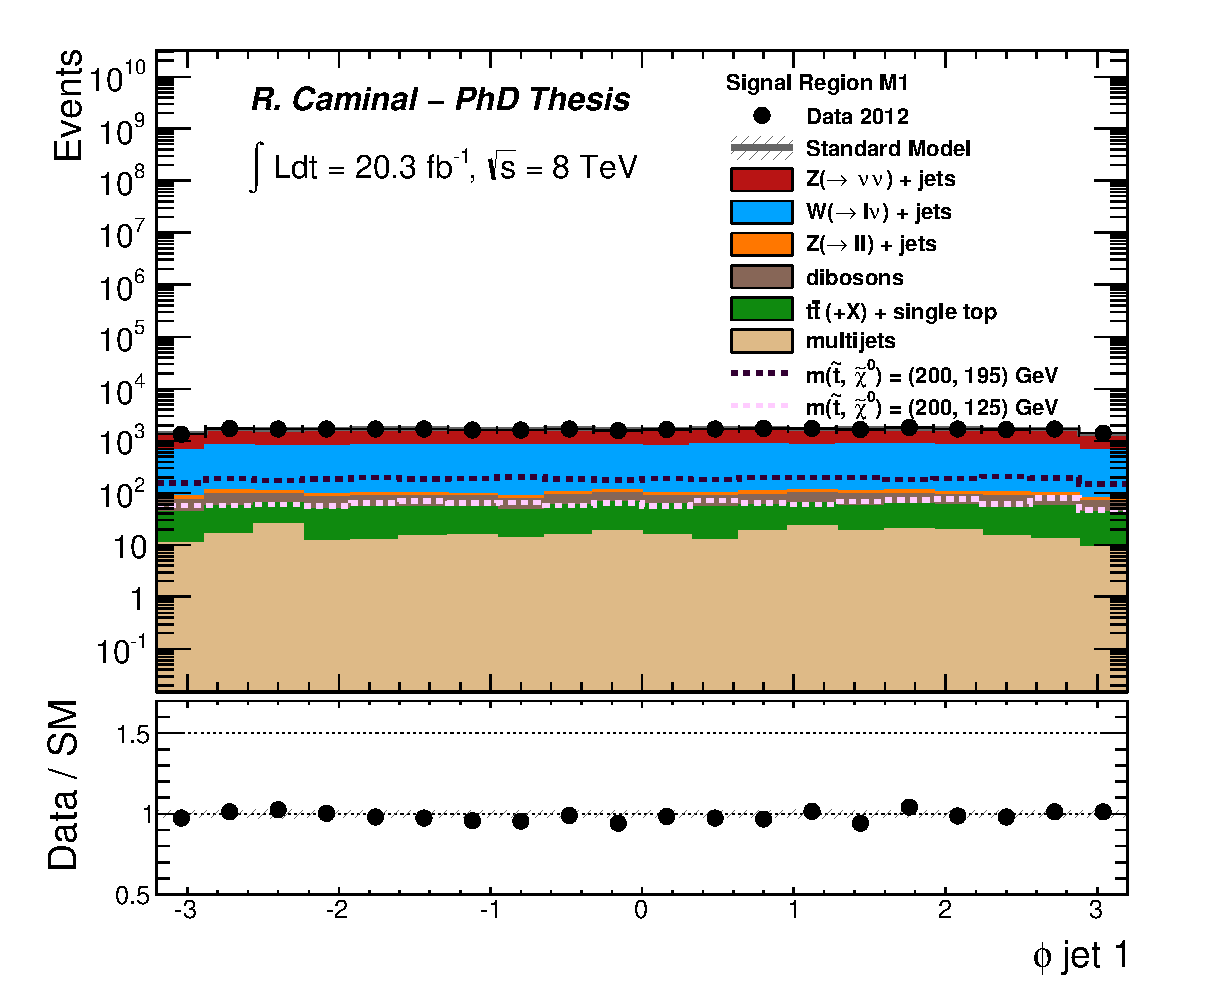
\includegraphics[width=0.495\textwidth]{MonojetAnalysis/Figures/plot_Stop_A6_SR_phi1_fitted.eps}
      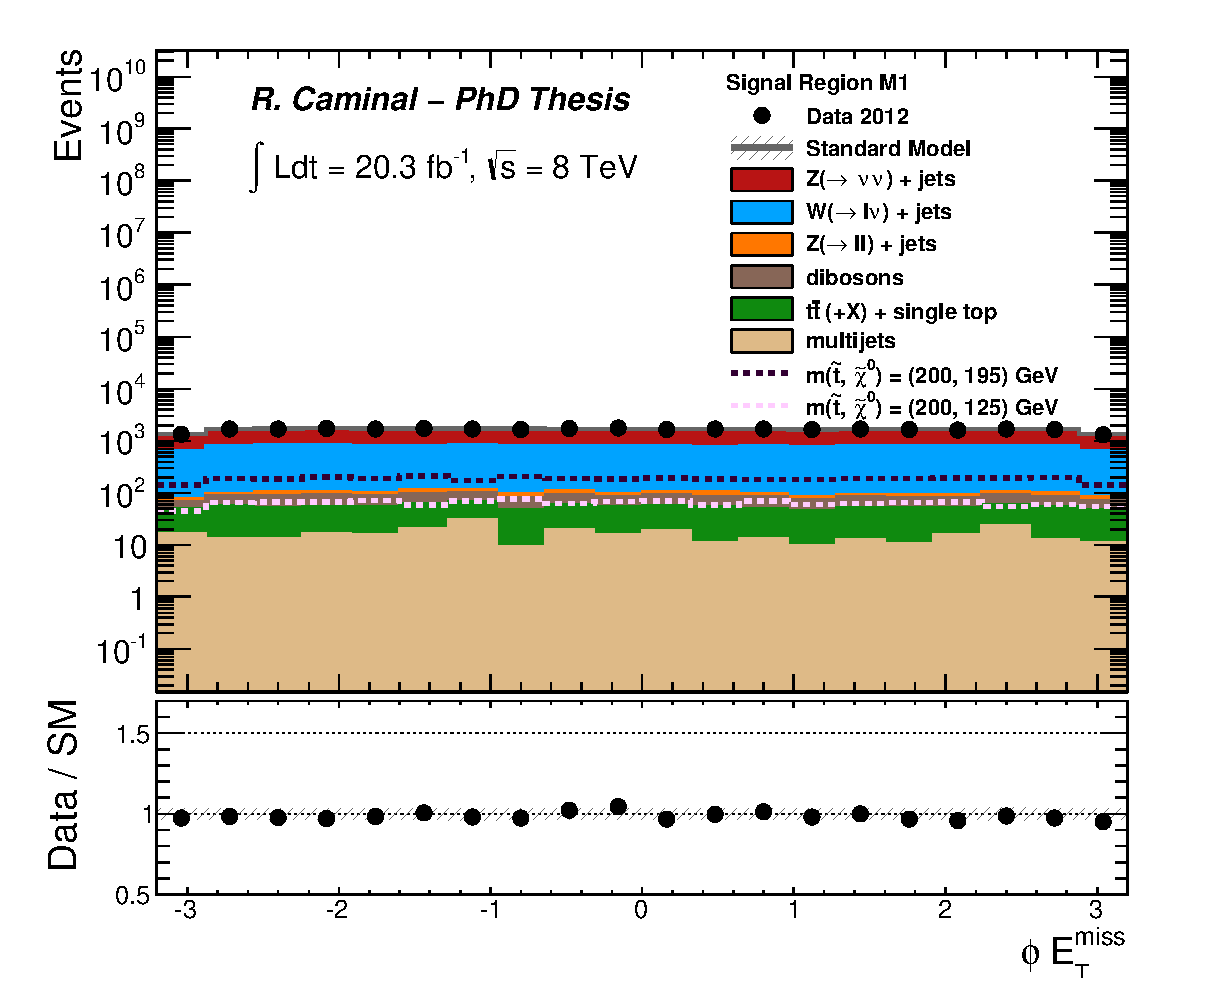
\includegraphics[width=0.495\textwidth]{MonojetAnalysis/Figures/plot_Stop_A6_SR_met_phi_fitted.eps}
    }
  \end{center}
  \caption[The measured azimutal angle, $\phi$, of the leading jet and the $\met$, for the selection cuts of region M1, after the normalization factors extracted from the fit have been applied.]
{The measured azimutal angle, $\phi$, of the leading jet (left) and the $\met$ (right), for the selection cuts M1, compared to the background predictions. The latter include the global normalization factors extracted from the fit. The error bands in the ratios include the statistical and experimental uncertainties on the background predictions. For illustration purposes, the distribution of two different SUSY scenarios for stop pair production are included.}
  \label{fig:Plot_M1_SR_Jet1_0}
\end{figure}

\begin{figure}[!ht]
  \begin{center}
    \mbox{
      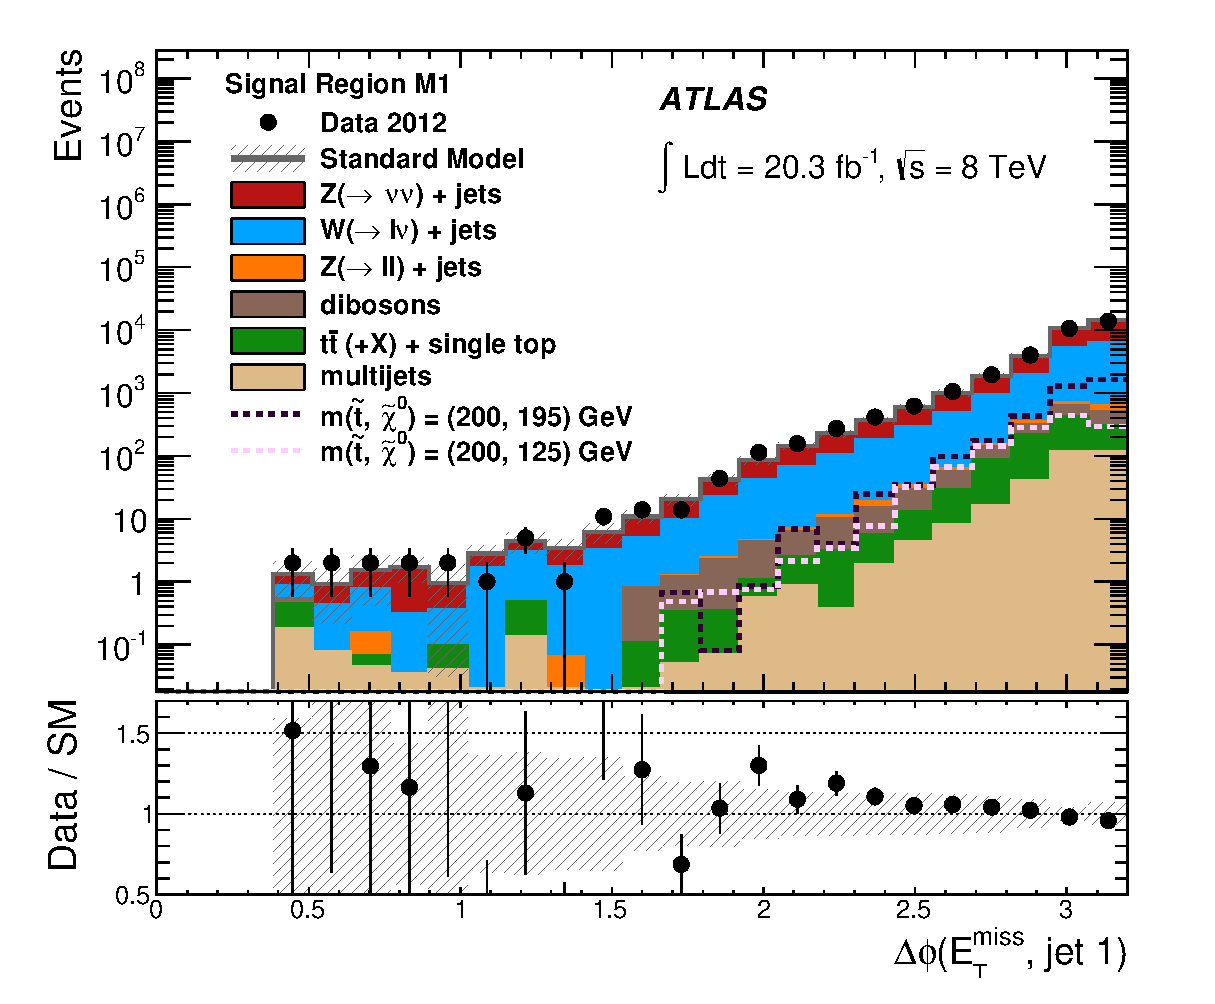
\includegraphics[width=0.495\textwidth]{MonojetAnalysis/Figures/plot_Stop_A6_SR_dPhi_met_j1_fitted.eps}
      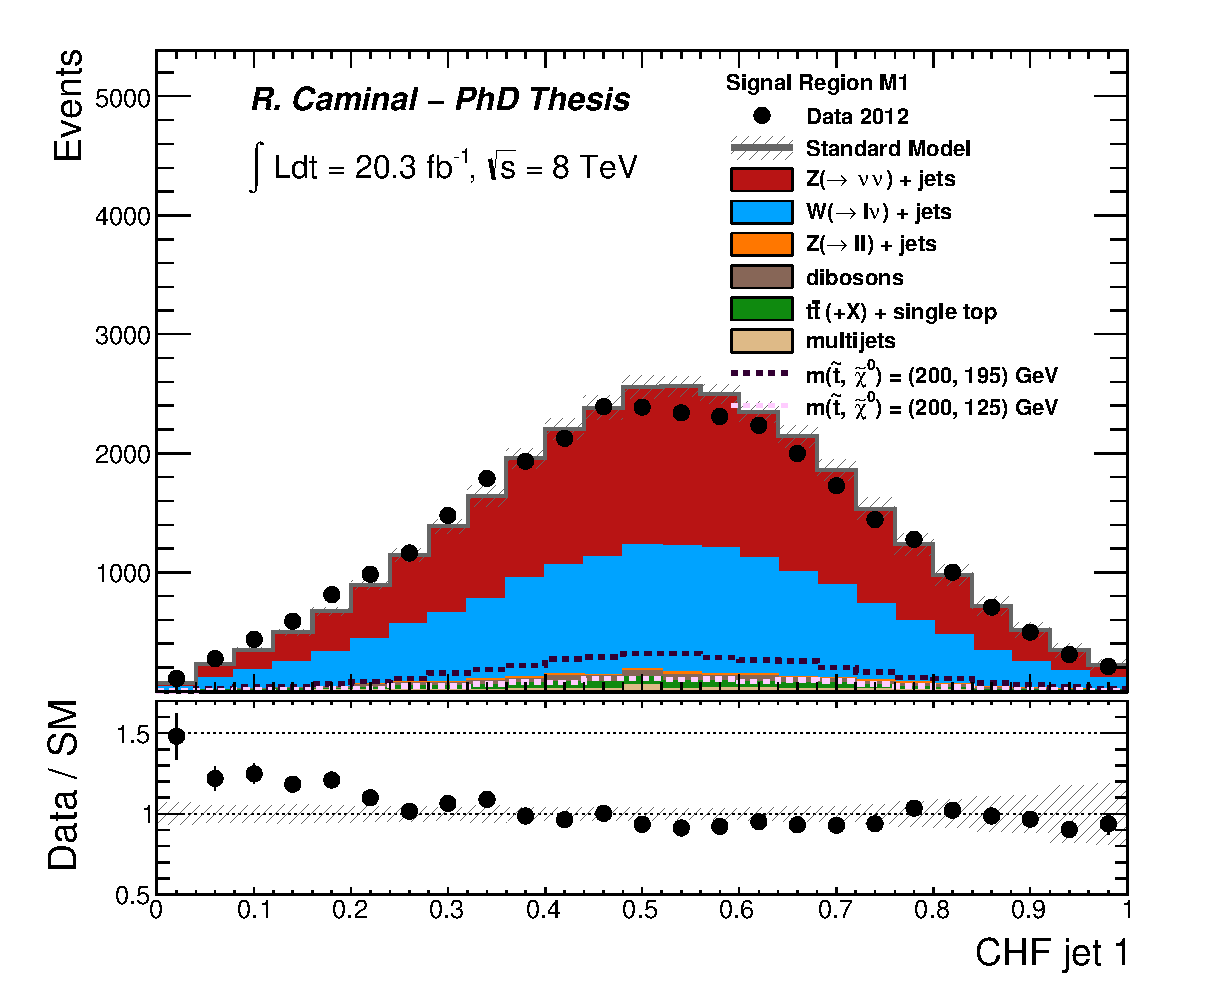
\includegraphics[width=0.495\textwidth]{MonojetAnalysis/Figures/plot_Stop_A6_SR_j1_chf_fitted.eps}
    }
  \end{center}
  \caption[Kinematic distributions of the $\Delta\phi(\met,\text{jet 1})$ and the charged fraction of the leading jet in the signal regions for the selection cuts of region M1, after the normalization factors extracted from the fit have been applied.]
{The measured azimutal angle difference between the leading jet and the $\met$ (left) and the charged fraction of the leading jet (right) in the signal regions for the selection cuts of region M1, compared to the background predictions. The latter include the global normalization factors extracted from the fit. The error bands in the ratios include the statistical and experimental uncertainties on the background predictions. For illustration purposes, the distribution of two different SUSY scenarios for stop pair production are included.}
  \label{fig:Plot_M1_SR_Jet1}
\end{figure}

\begin{figure}[!ht]
  \begin{center}
    \mbox{
      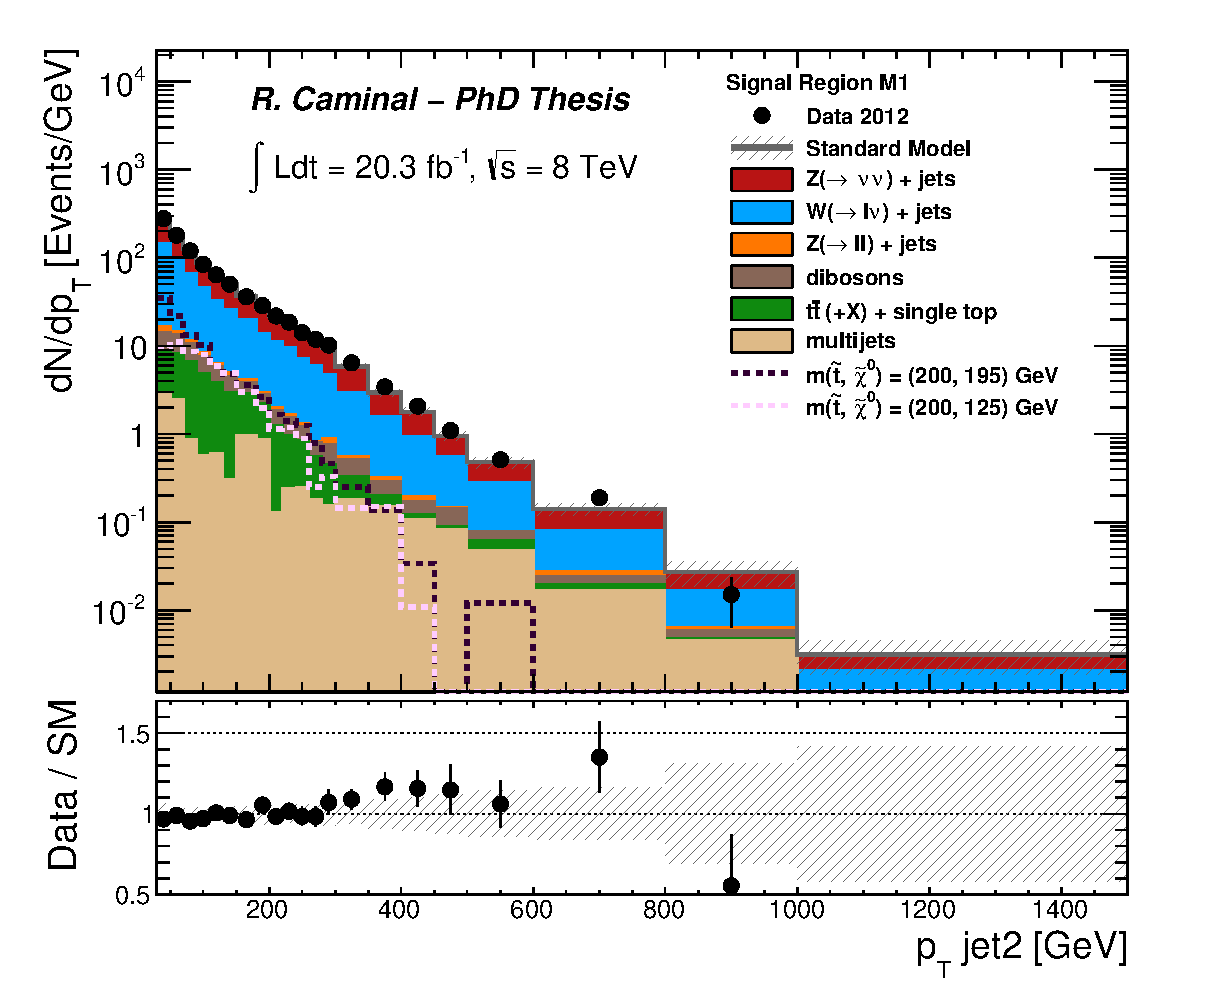
\includegraphics[width=0.495\textwidth]{MonojetAnalysis/Figures/plot_Stop_A6_SR_pt2_fitted.eps}
      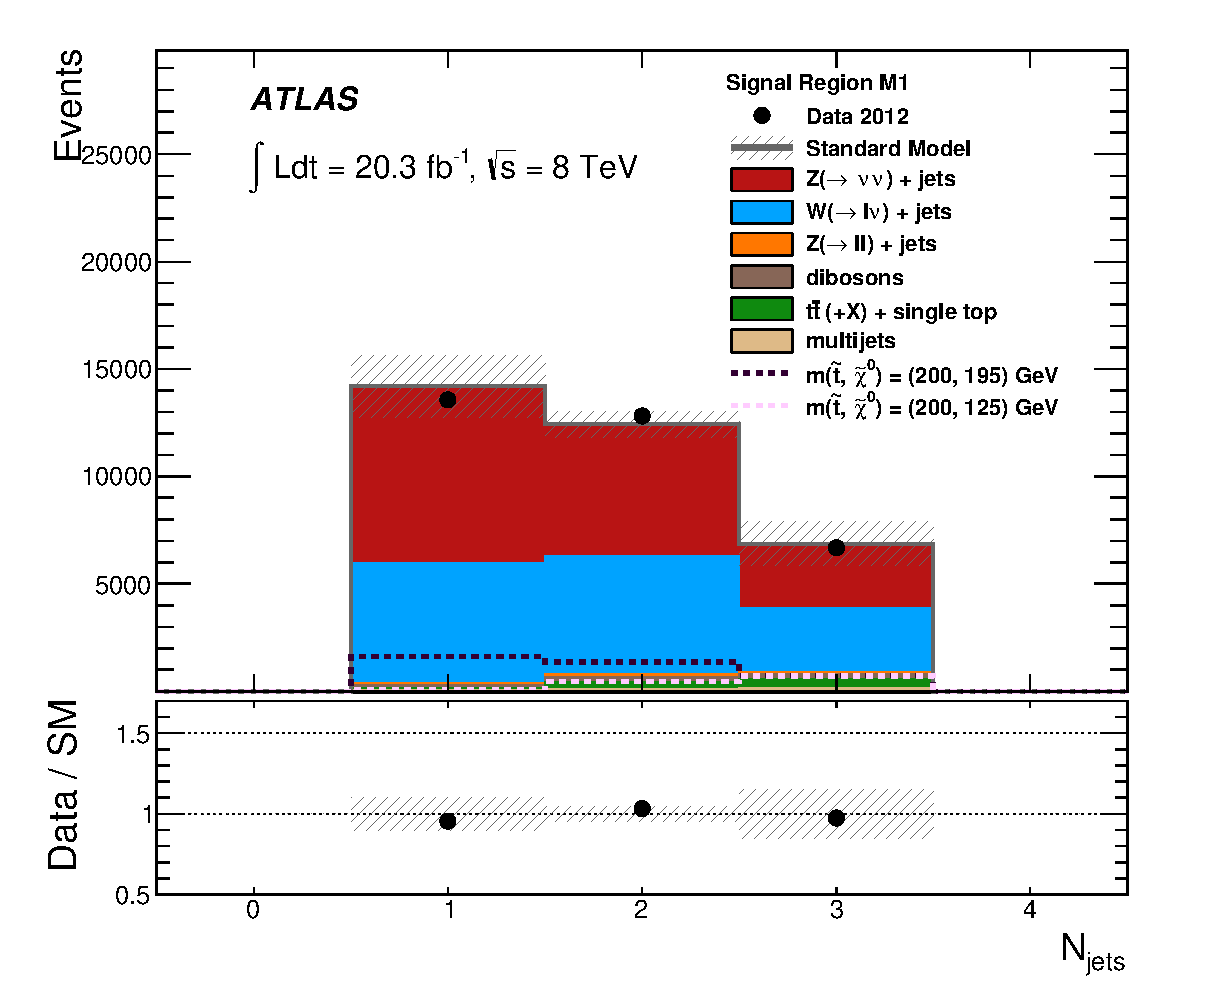
\includegraphics[width=0.495\textwidth]{MonojetAnalysis/Figures/plot_Stop_A6_SR_n_jets_fitted.eps}
    }
    \mbox{
      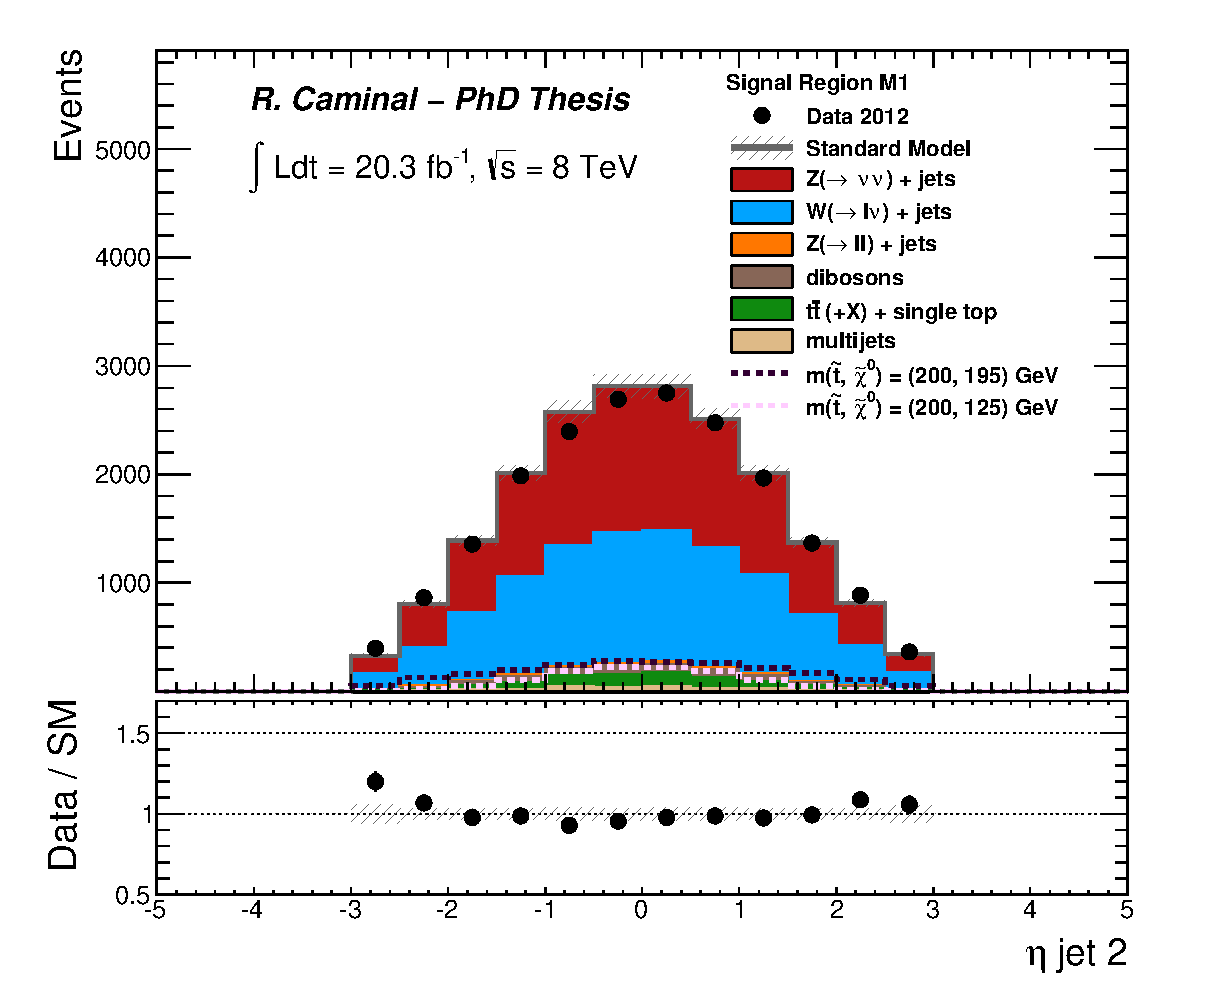
\includegraphics[width=0.495\textwidth]{MonojetAnalysis/Figures/plot_Stop_A6_SR_eta2_fitted.eps}
      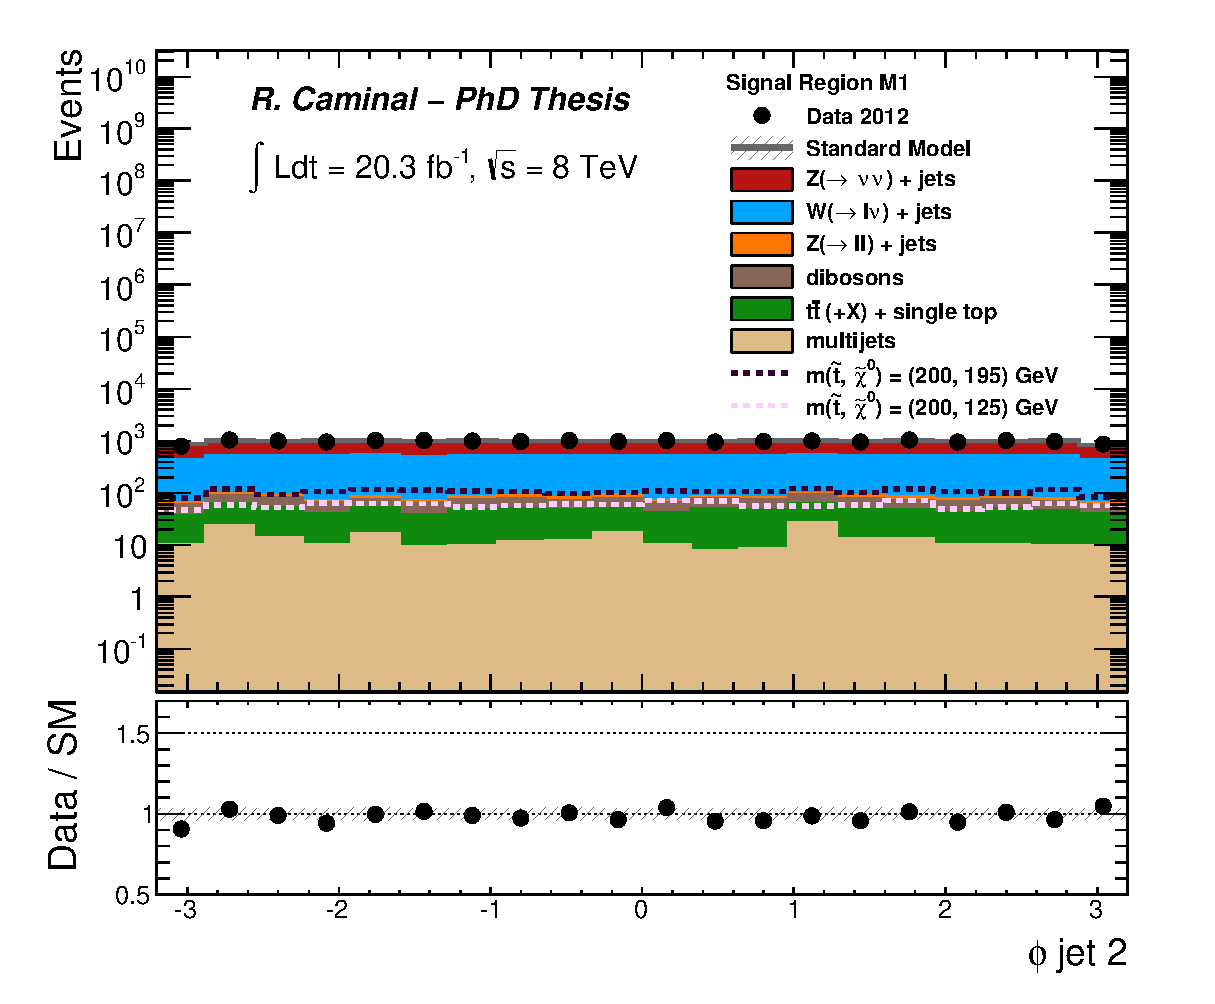
\includegraphics[width=0.495\textwidth]{MonojetAnalysis/Figures/plot_Stop_A6_SR_phi2_fitted.eps}
    }
  \end{center}
  \caption[Kinematic distributions of the $\pt$ of the second leading jet, the jet multiplicity, and the pseudo-rapidity and azimutal angle of the second leading jet in the signal regions for the selection cuts of region M1, after the normalization factors extracted from the fit have been applied.]
{The measured $\pt$ of the second leading jet (top left), the jet multiplicity (top right), and the pseudo-rapidity (bottom left) and azimutal angle (bottom right) of the second leading jet in the signal regions for the selection cuts of region M1, compared to the background predictions. The latter include the global normalization factors extracted from the fit. The error bands in the ratios include the statistical and experimental uncertainties on the background predictions. For illustration purposes, the distribution of two different SUSY scenarios for stop pair production are included.}
  \label{fig:Plot_M1_SR_Jet2}
\end{figure}

\begin{figure}[!ht]
  \begin{center}
    \mbox{
      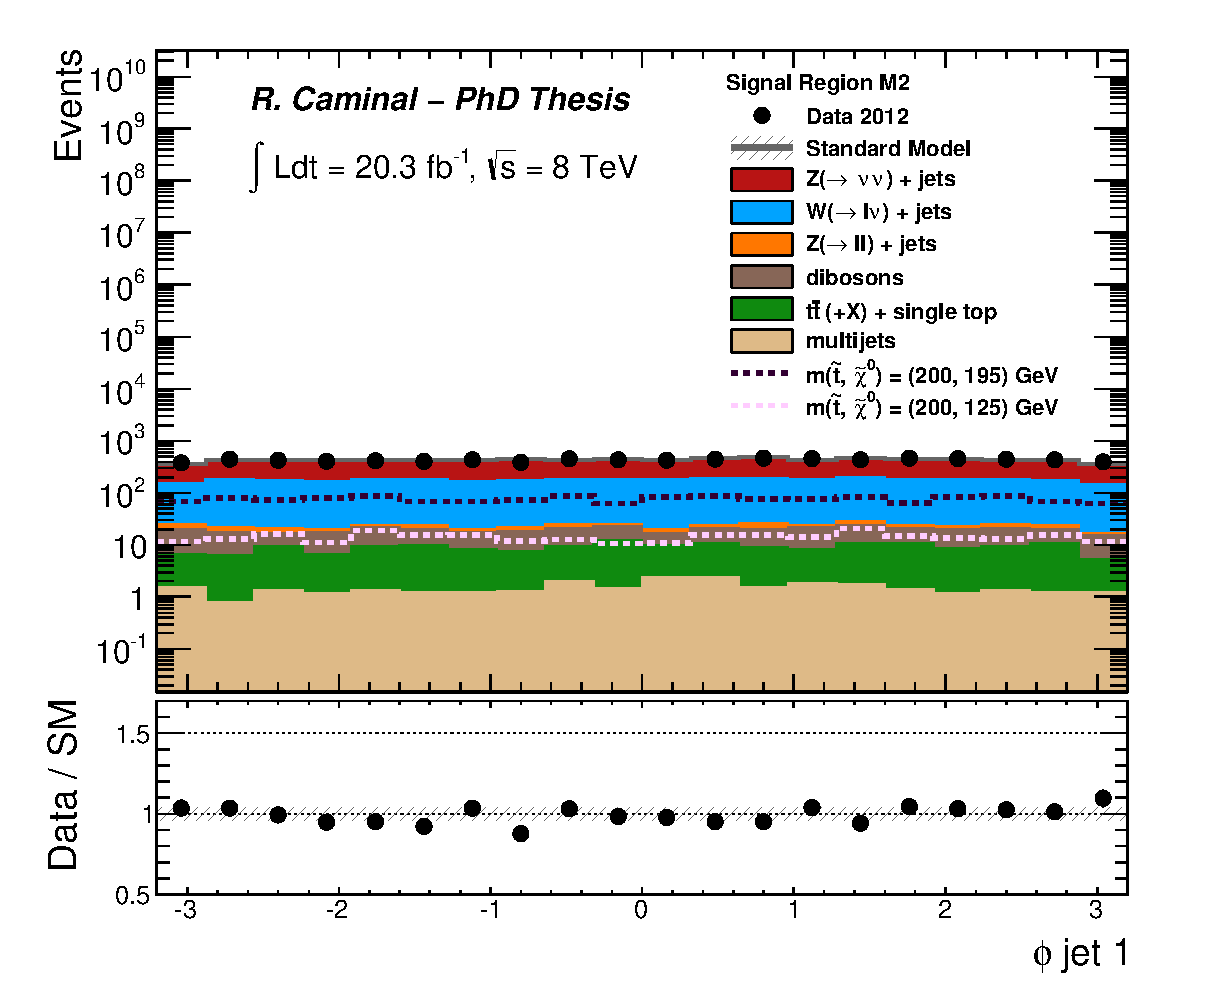
\includegraphics[width=0.495\textwidth]{MonojetAnalysis/Figures/plot_Stop_A3_SR_phi1_fitted.eps}
      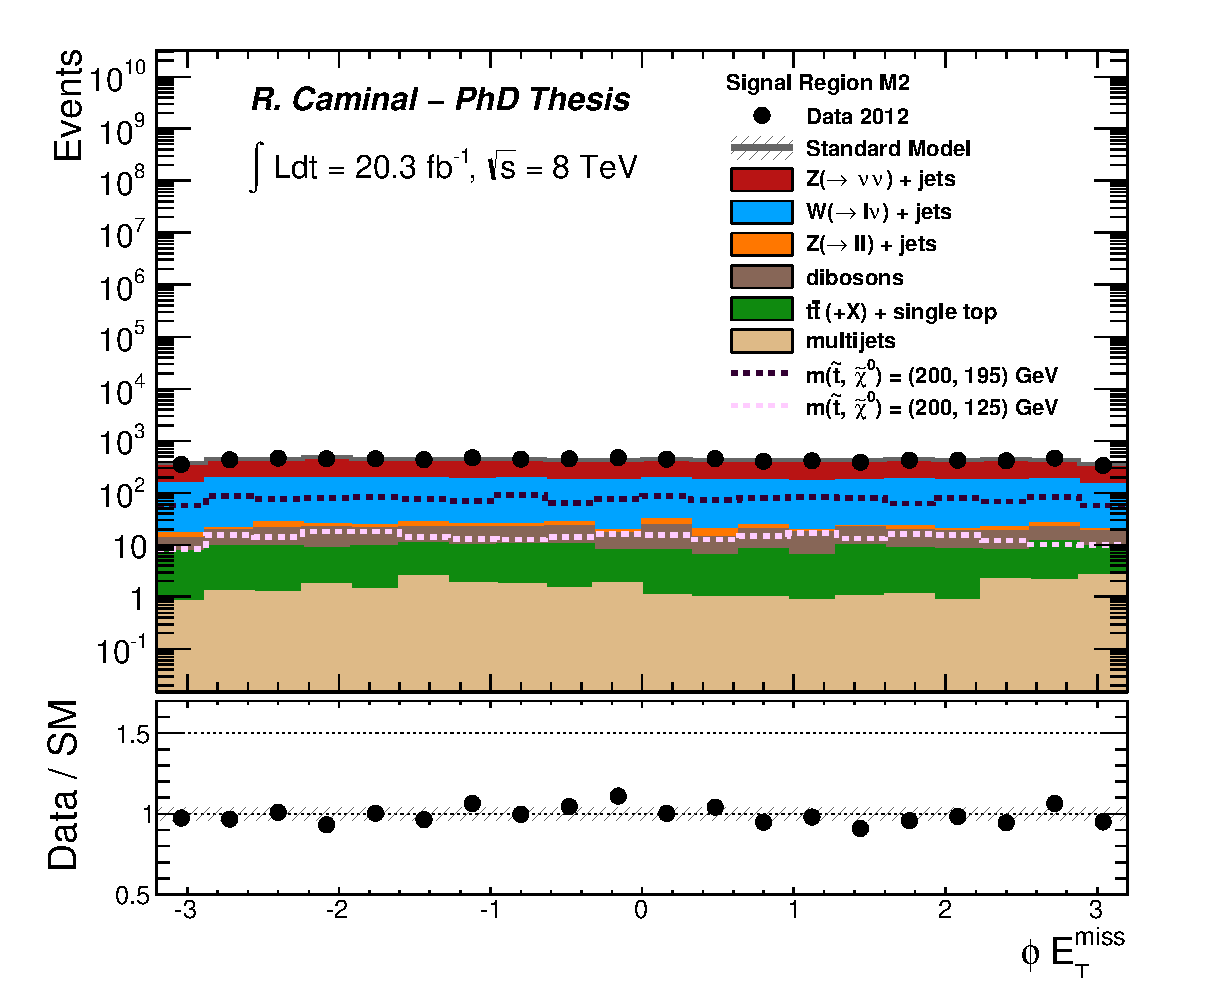
\includegraphics[width=0.495\textwidth]{MonojetAnalysis/Figures/plot_Stop_A3_SR_met_phi_fitted.eps}
    }
    \mbox{
      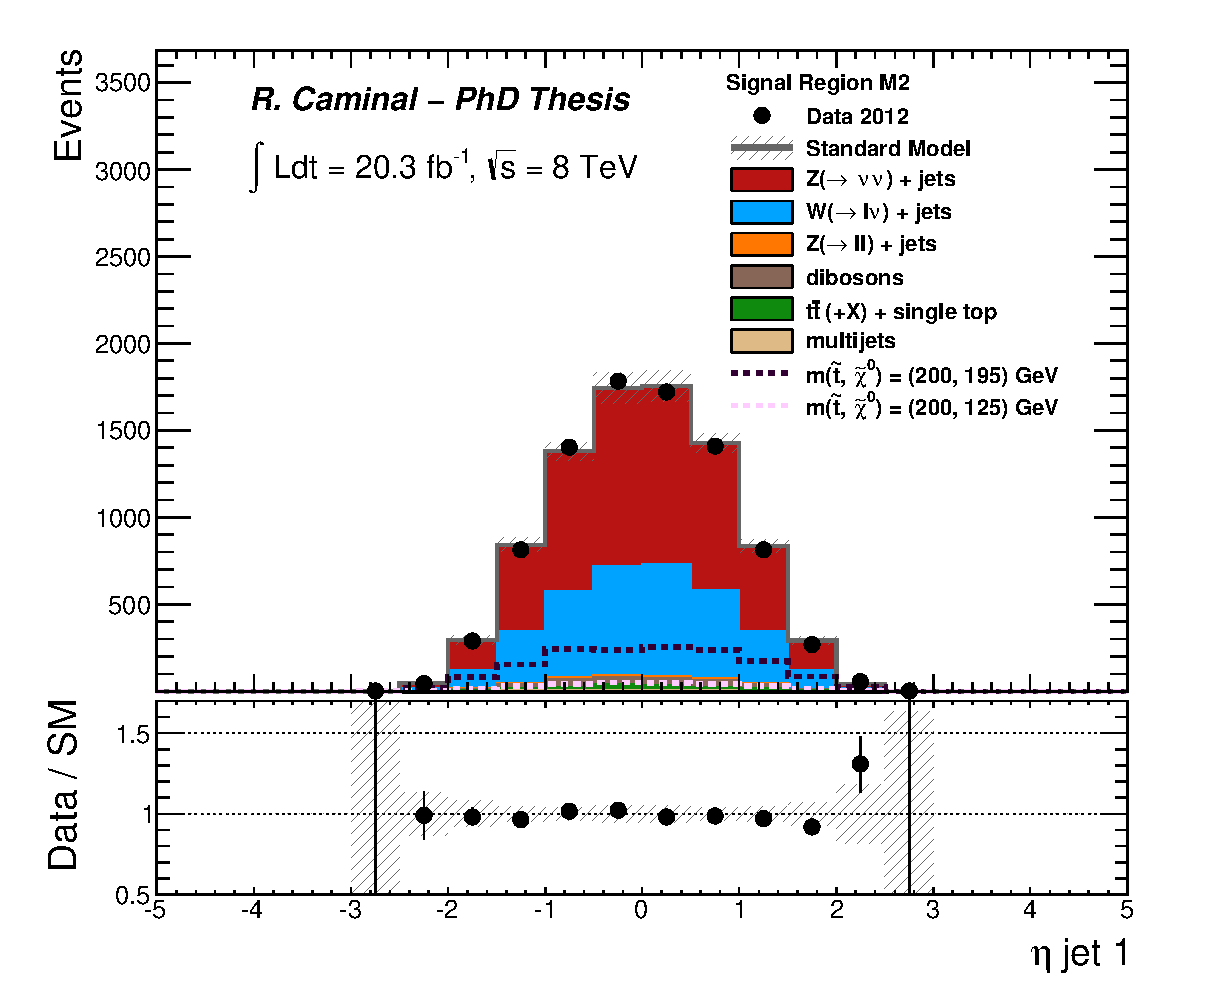
\includegraphics[width=0.495\textwidth]{MonojetAnalysis/Figures/plot_Stop_A3_SR_eta1_fitted.eps}
      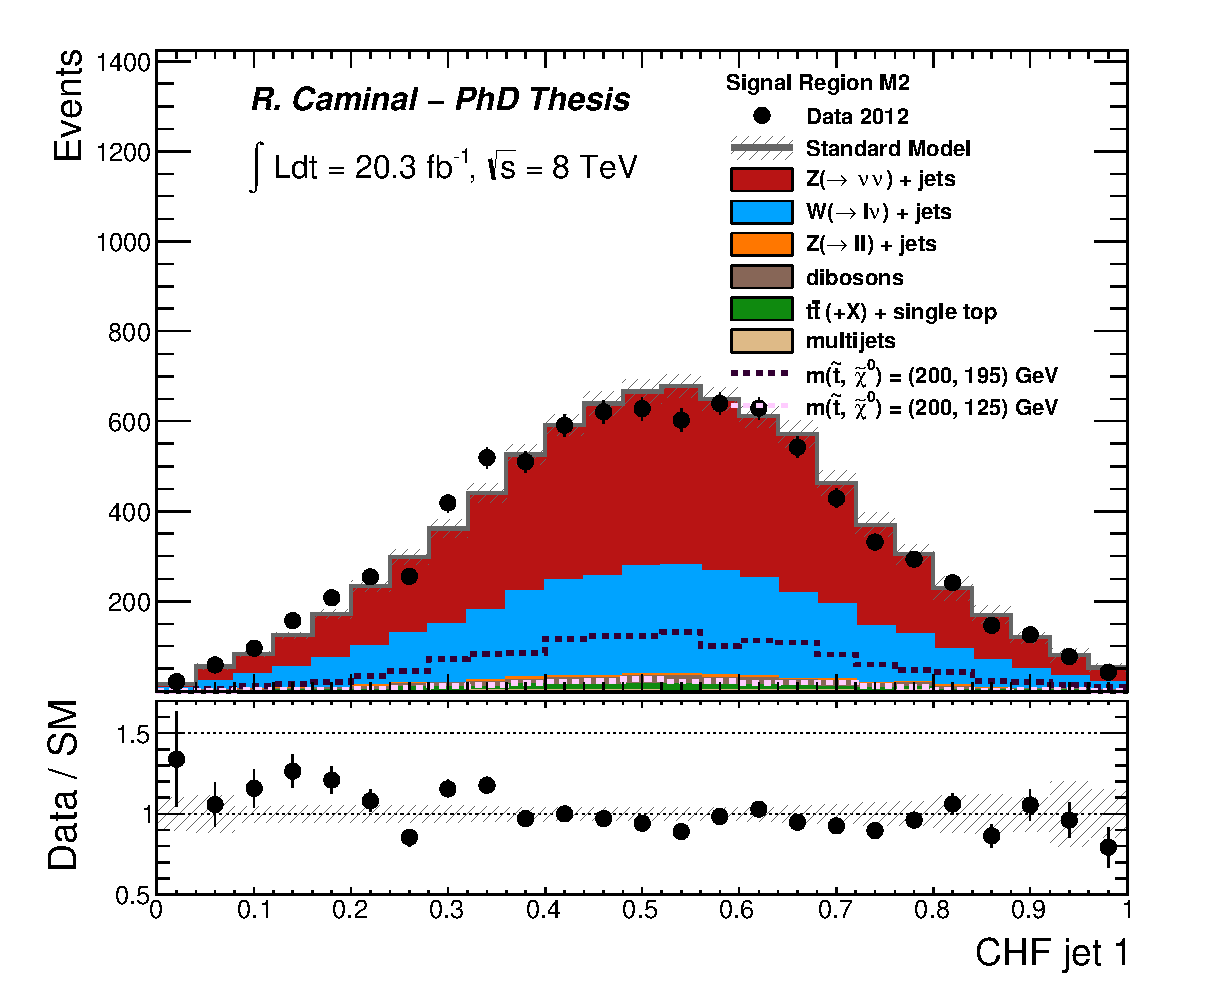
\includegraphics[width=0.495\textwidth]{MonojetAnalysis/Figures/plot_Stop_A3_SR_j1_chf_fitted.eps}
    }
  \end{center}
  \caption[Kinematic distributions of the azimutal angle, $\phi$, of the leading jet and the missing transverse energy, the azimutal angle difference between the leading jet and the $\met$, and the charge fraction of the leading jet in the signal regions for the selection cuts of region M2, after the normalization factors extracted from the fit have been applied.]
{The measured azimutal angle, $\phi$, of the leading jet (top left) and the missing transverse energy (top right), the azimutal angle difference between the leading jet and the $\met$ (bottom left) and the charge fraction of the leading jet (bottom right) for the selection cuts M2, compared to the background predictions. The latter include the global normalization factors extracted from the fit. The error bands in the ratios include the statistical and experimental uncertainties on the background predictions. For illustration purposes, the distribution of two different SUSY scenarios for stop pair production are included.}
  \label{fig:Plot_M2_SR_Jet1}
\end{figure}

\begin{figure}[!ht]
  \begin{center}
    \mbox{
      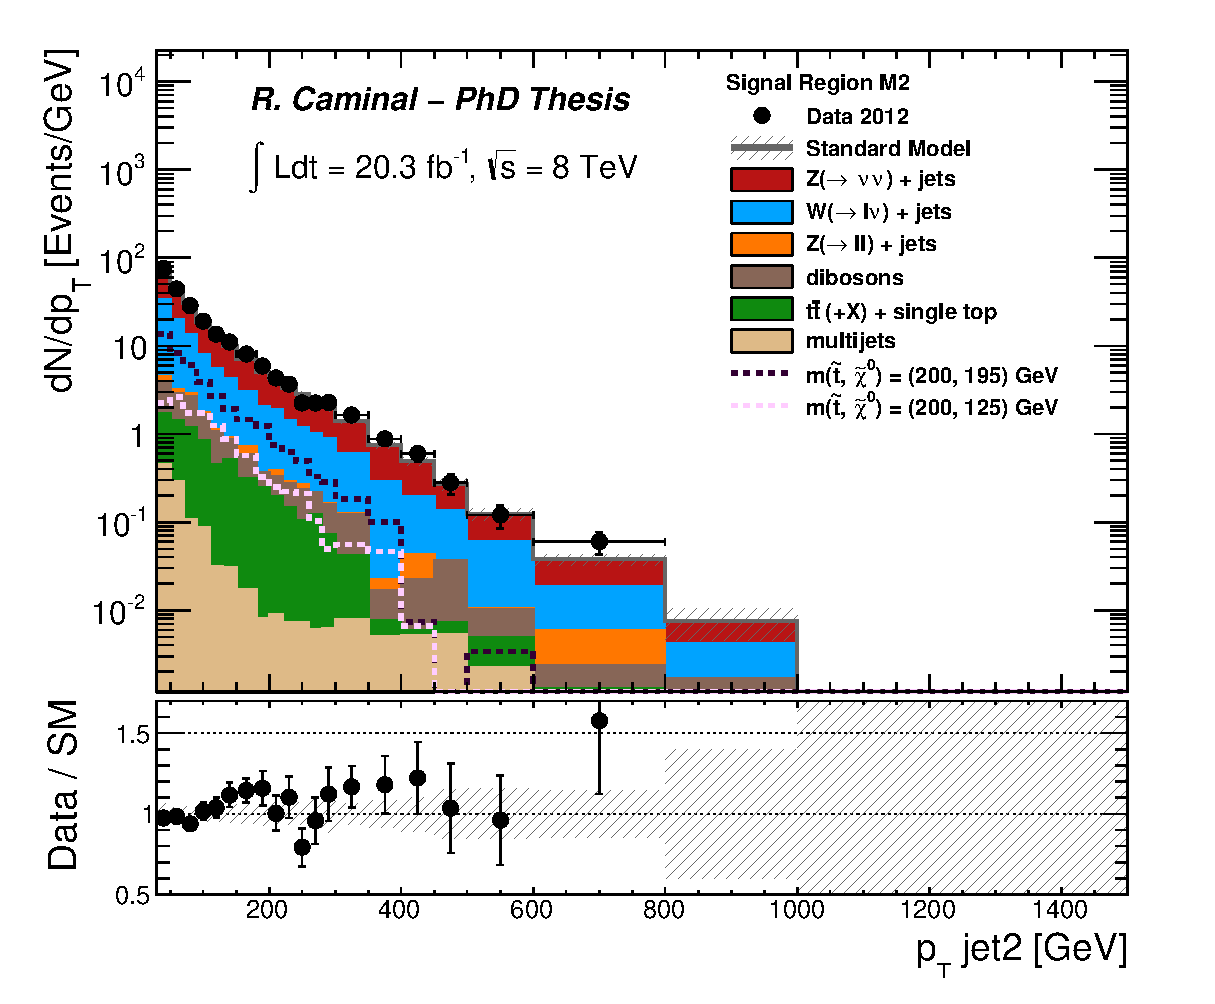
\includegraphics[width=0.495\textwidth]{MonojetAnalysis/Figures/plot_Stop_A3_SR_pt2_fitted.eps}
      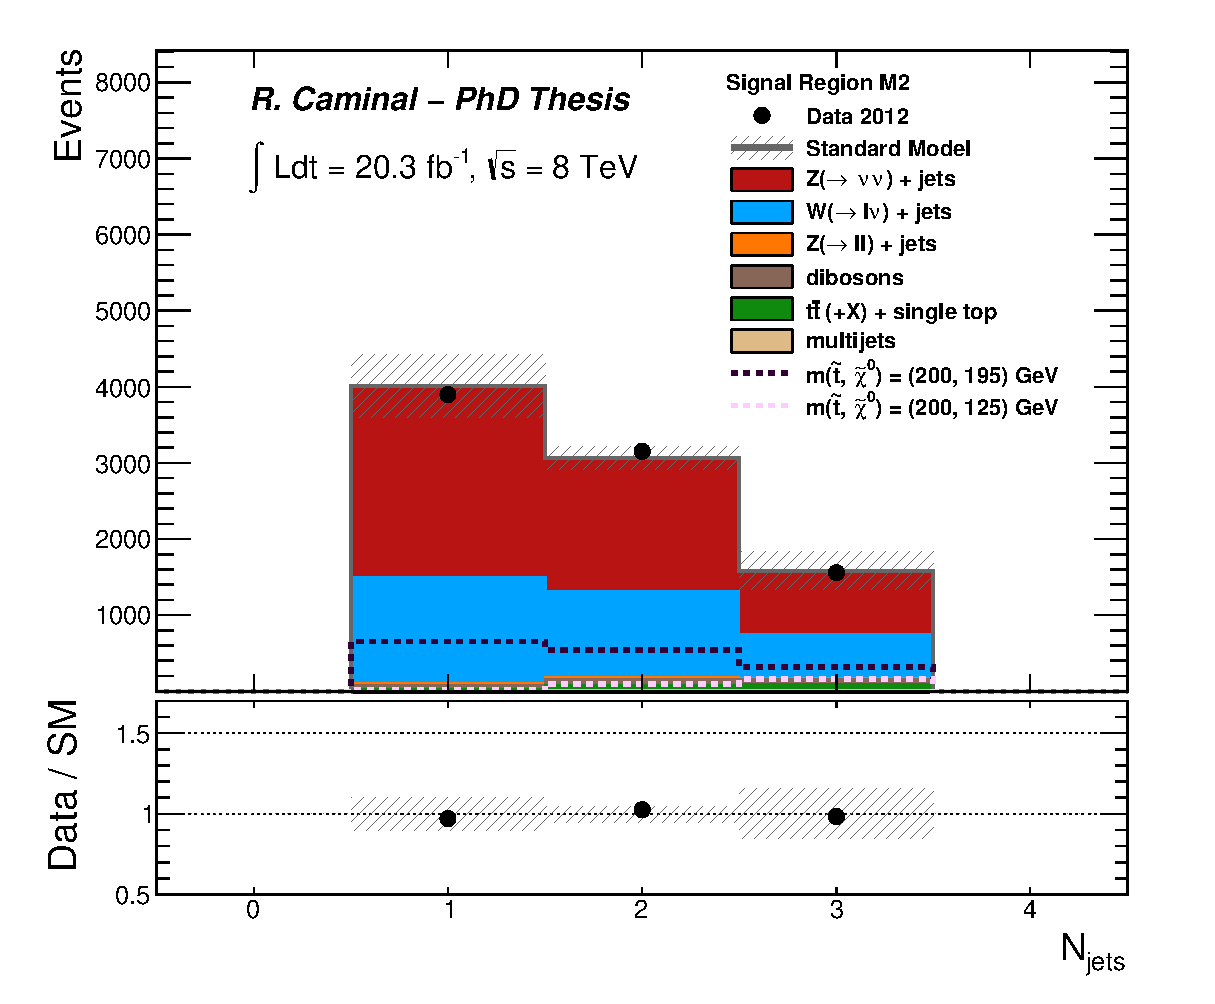
\includegraphics[width=0.495\textwidth]{MonojetAnalysis/Figures/plot_Stop_A3_SR_n_jets_fitted.eps}
    }
    \mbox{
      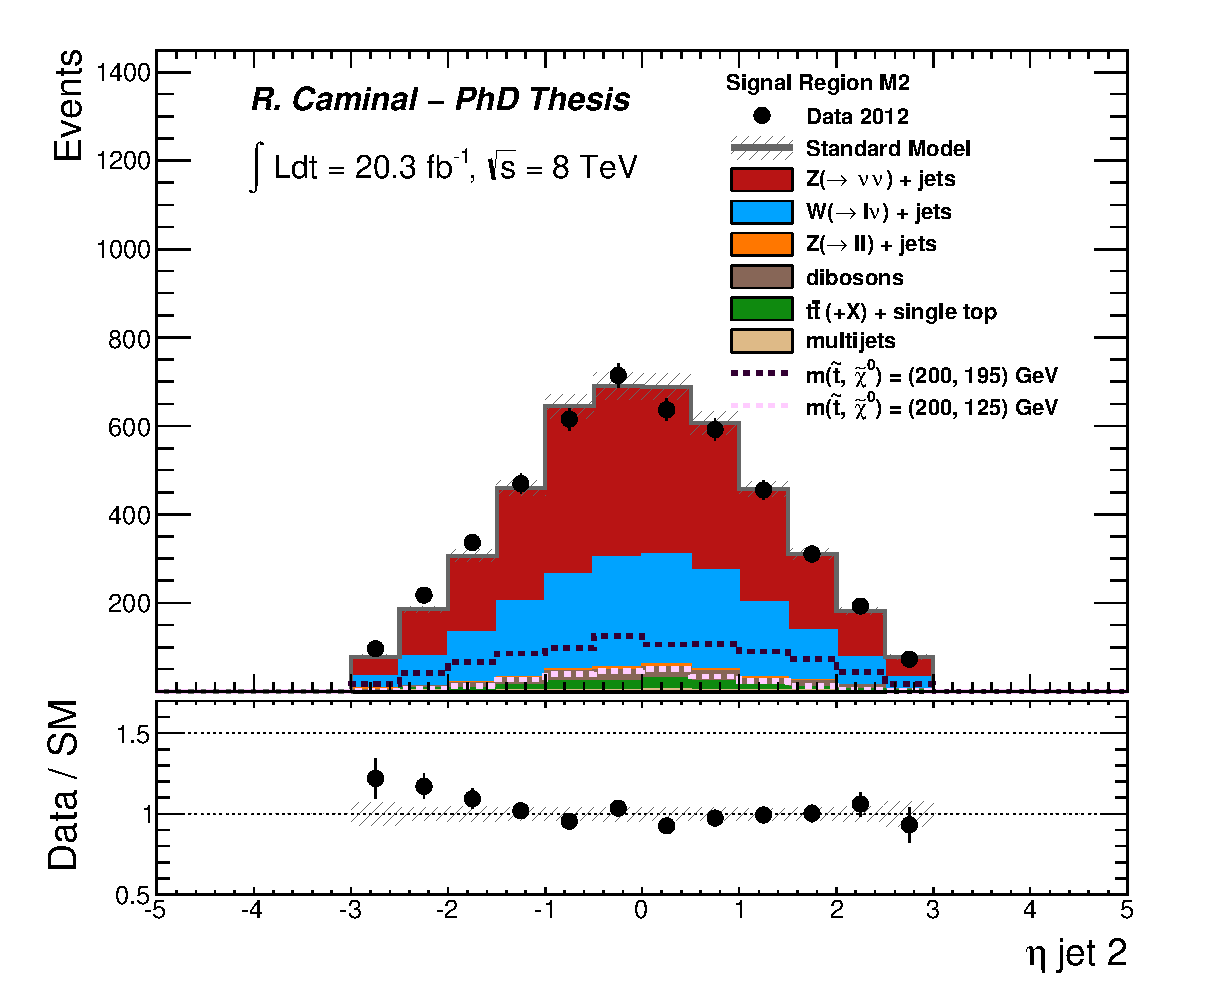
\includegraphics[width=0.495\textwidth]{MonojetAnalysis/Figures/plot_Stop_A3_SR_eta2_fitted.eps}
      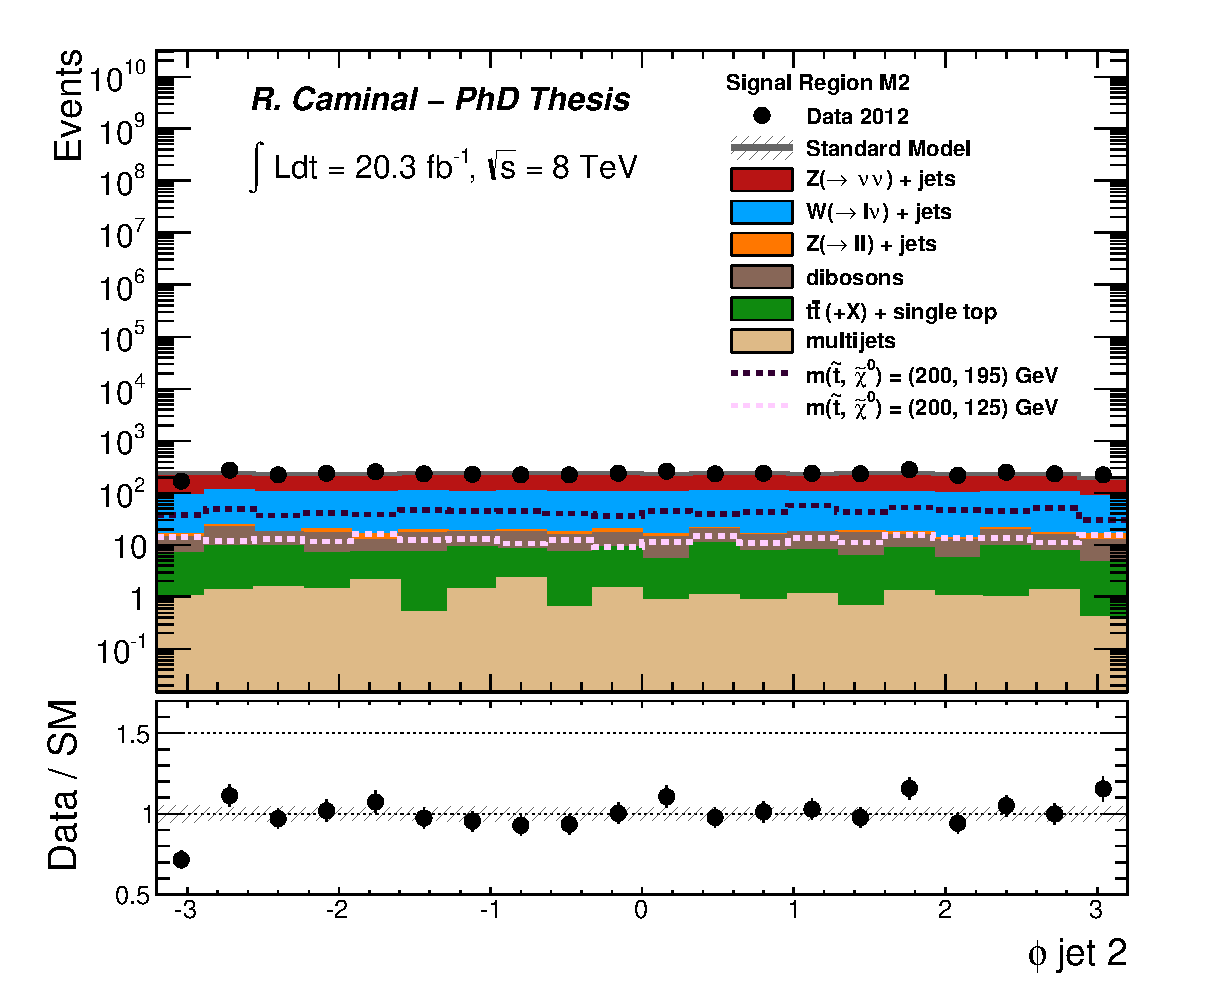
\includegraphics[width=0.495\textwidth]{MonojetAnalysis/Figures/plot_Stop_A3_SR_phi2_fitted.eps}
    }
  \end{center}
  \caption[Kinematic distributions of the $\pt$ of the second leading jet, the jet multiplicity, and the pseudo-rapidity and azimutal angle of the second leading jet in the signal regions for the selection cuts of region M2, after the normalization factors extracted from the fit have been applied.]
{The measured $\pt$ of the second leading jet (top left), the jet multiplicity (top right), and the pseudo-rapidity (bottom left) and azimutal angle (bottom right) of the second leading jet in the signal regions for the selection cuts of region M2, compared to the background predictions. The latter include the global normalization factors extracted from the fit. The error bands in the ratios include the statistical and experimental uncertainties on the background predictions. For illustration purposes, the distribution of two different SUSY scenarios for stop pair production are included.}
  \label{fig:Plot_M2_SR_Jet2}
\end{figure}

\begin{figure}[!ht]
  \begin{center}
    \mbox{
      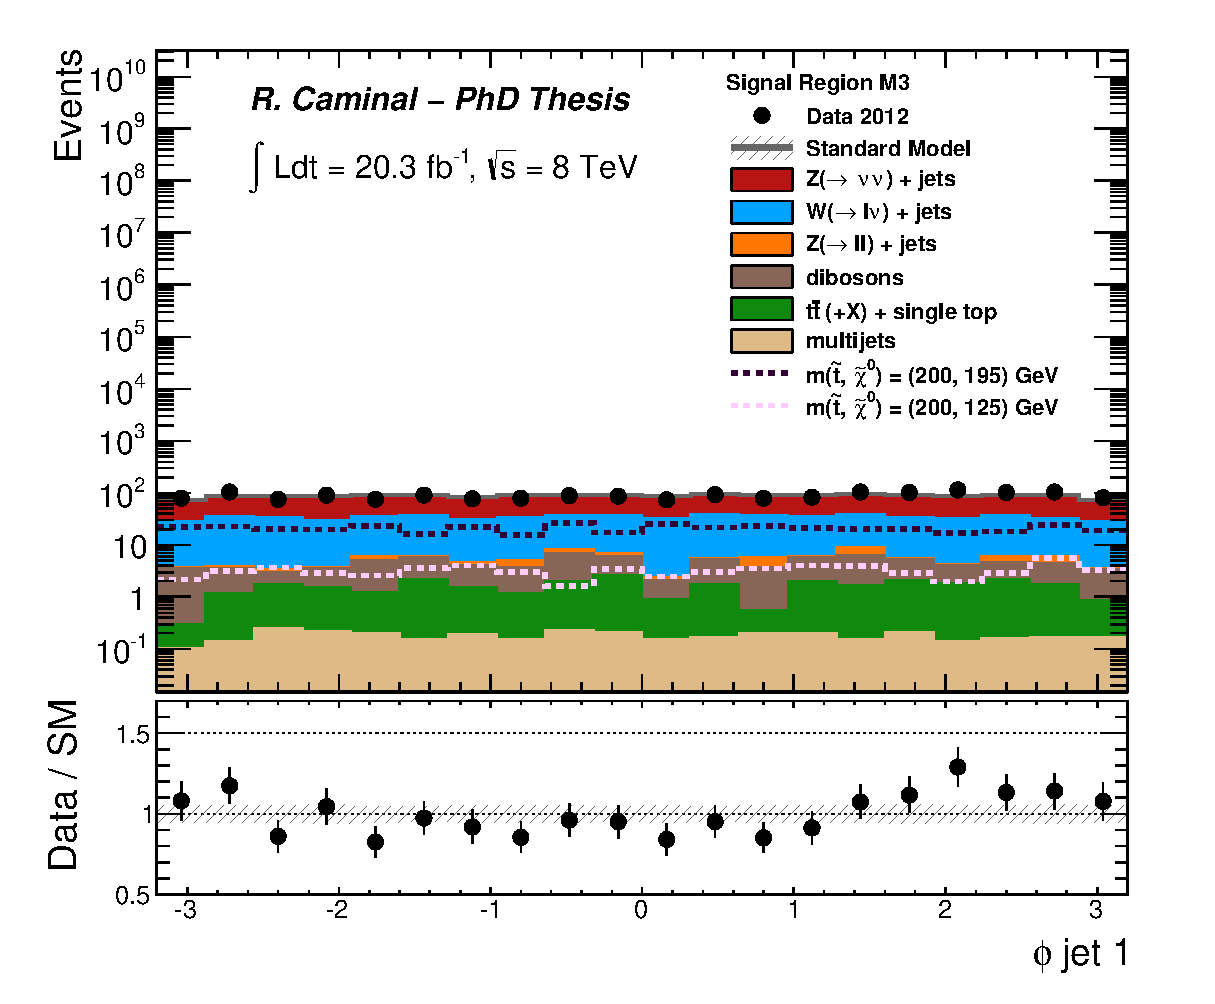
\includegraphics[width=0.495\textwidth]{MonojetAnalysis/Figures/plot_Stop_A4_SR_phi1_fitted.eps}
      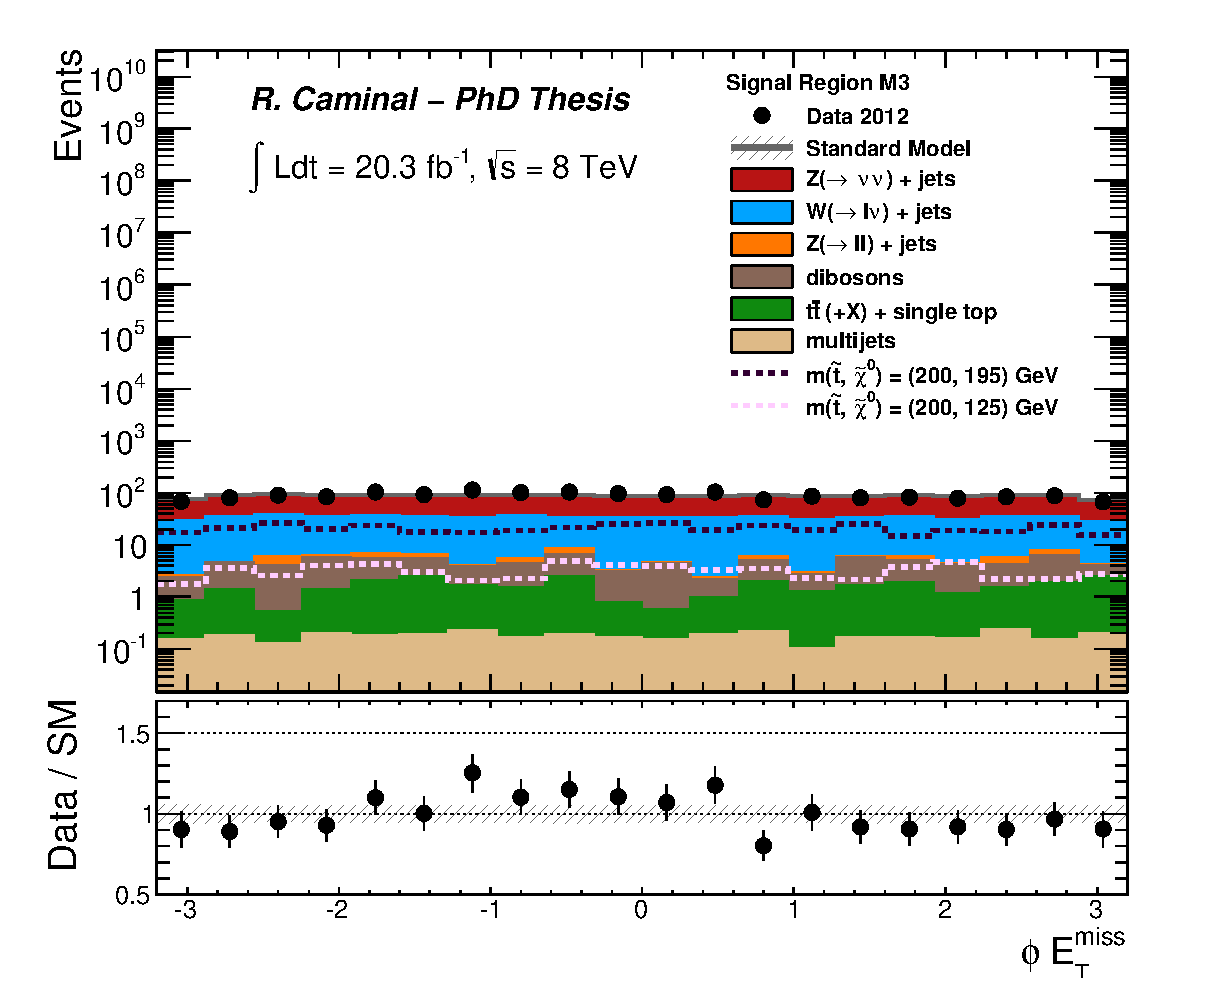
\includegraphics[width=0.495\textwidth]{MonojetAnalysis/Figures/plot_Stop_A4_SR_met_phi_fitted.eps}
    }
    \mbox{
      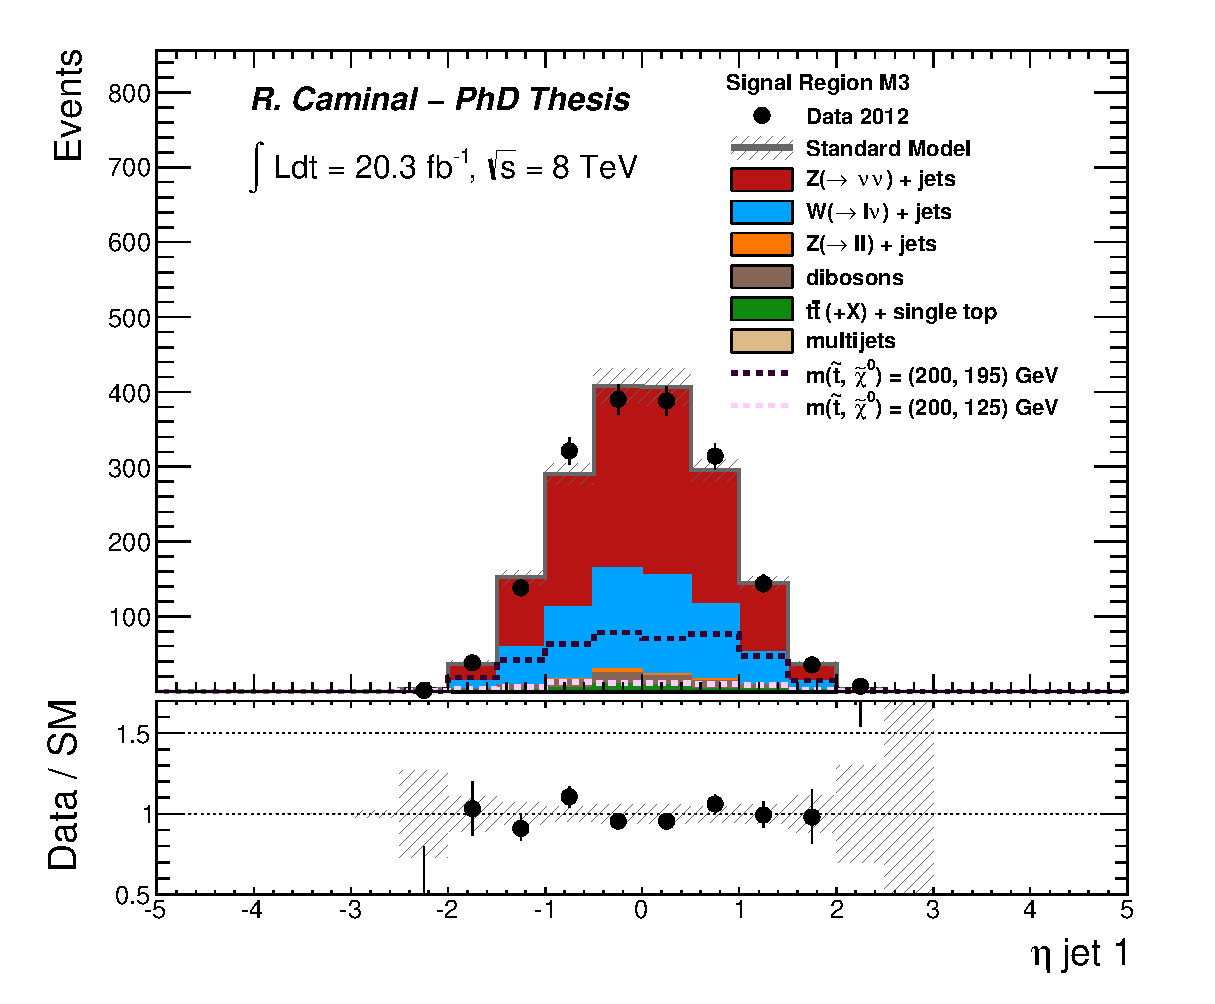
\includegraphics[width=0.495\textwidth]{MonojetAnalysis/Figures/plot_Stop_A4_SR_eta1_fitted.eps}
      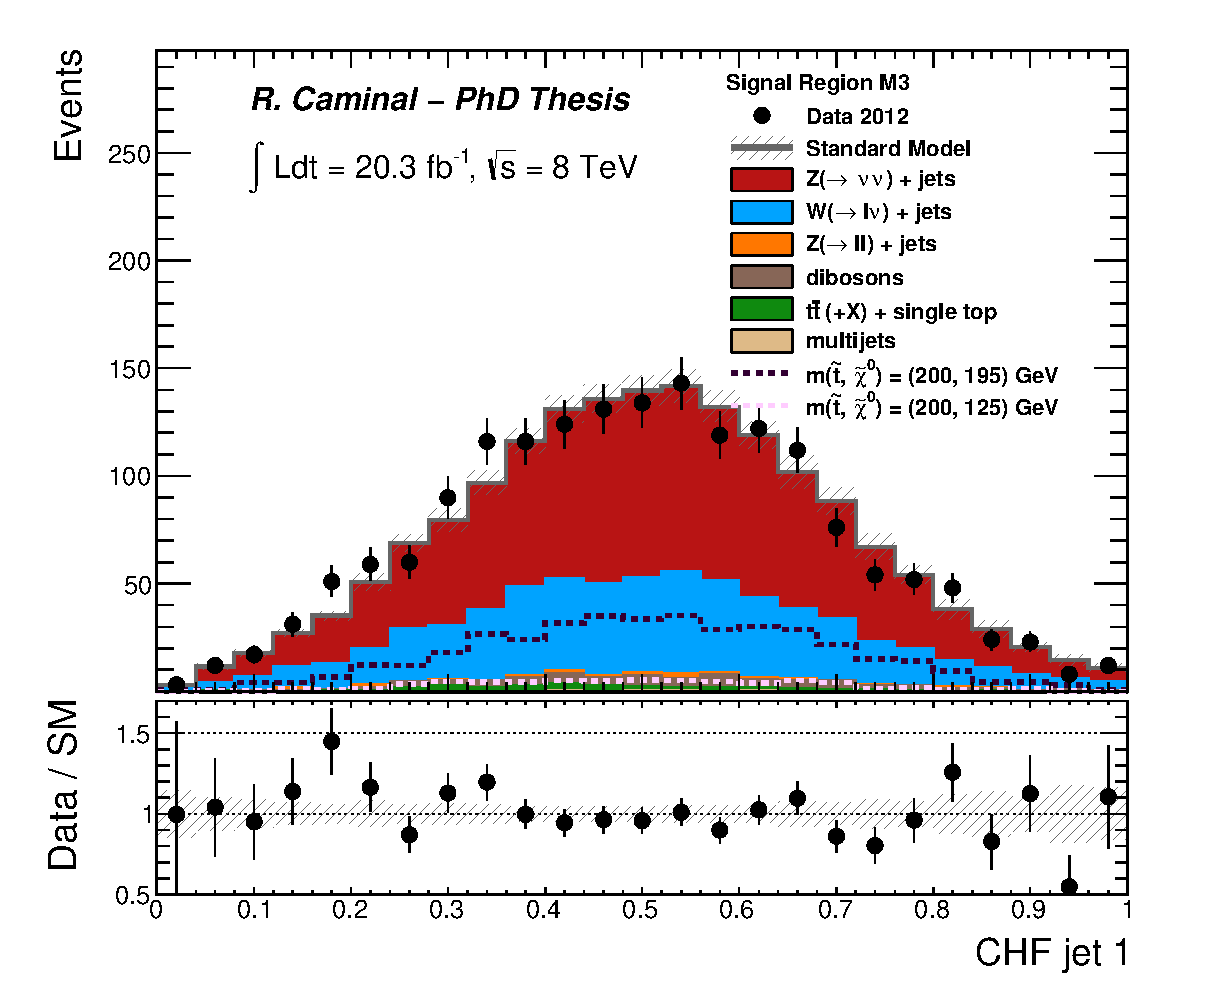
\includegraphics[width=0.495\textwidth]{MonojetAnalysis/Figures/plot_Stop_A4_SR_j1_chf_fitted.eps}
    }
  \end{center}
  \caption[Kinematic distributions of the azimutal angle, $\phi$, of the leading jet and the missing transverse energy, the azimutal angle difference between the leading jet and the $\met$, and the charge fraction of the leading jet in the signal regions for the selection cuts of region M3, after the normalization factors extracted from the fit have been applied.]
{The measured azimutal angle, $\phi$, of the leading jet (top left) and the missing transverse energy (top right), the azimutal angle difference between the leading jet and the $\met$ (bottom left) and the charge fraction of the leading jet (bottom right) for the selection cuts M3, compared to the background predictions. The latter include the global normalization factors extracted from the fit. The error bands in the ratios include the statistical and experimental uncertainties on the background predictions. For illustration purposes, the distribution of two different SUSY scenarios for stop pair production are included.}
  \label{fig:Plot_M3_SR_Jet1}
\end{figure}

\begin{figure}[!ht]
  \begin{center}
    \mbox{
      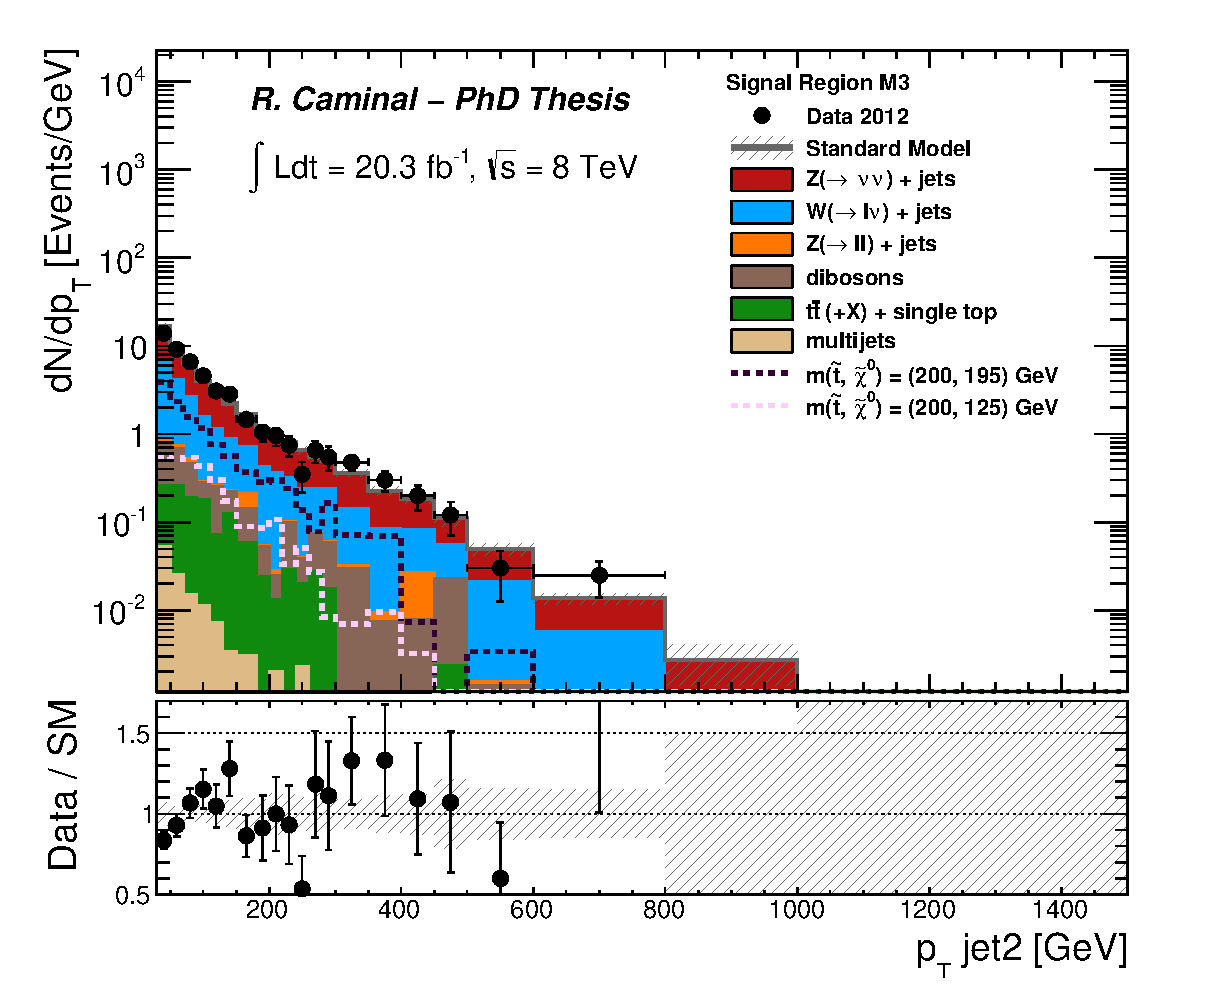
\includegraphics[width=0.495\textwidth]{MonojetAnalysis/Figures/plot_Stop_A4_SR_pt2_fitted.eps}
      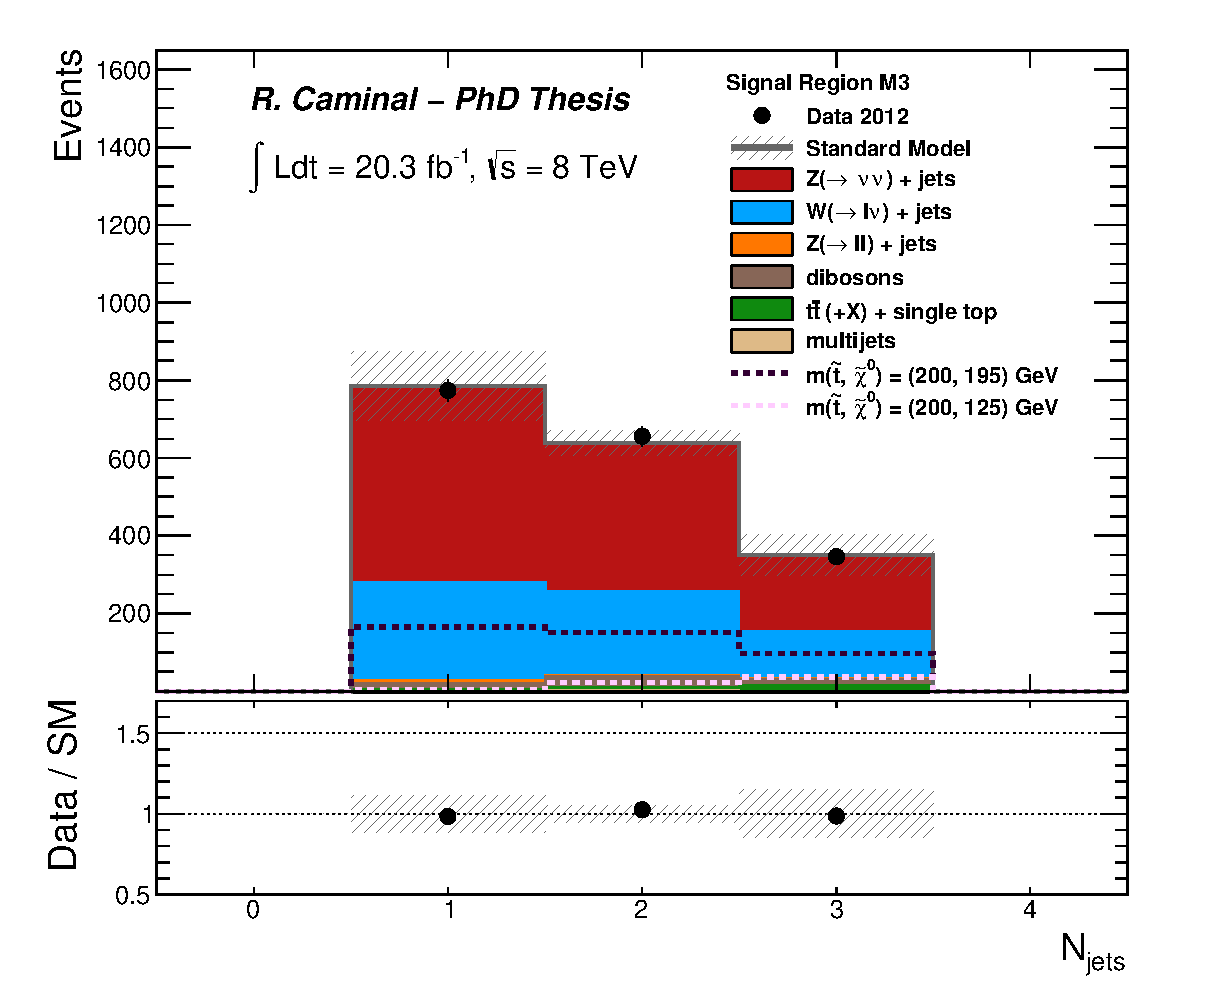
\includegraphics[width=0.495\textwidth]{MonojetAnalysis/Figures/plot_Stop_A4_SR_n_jets_fitted.eps}
    }
    \mbox{
      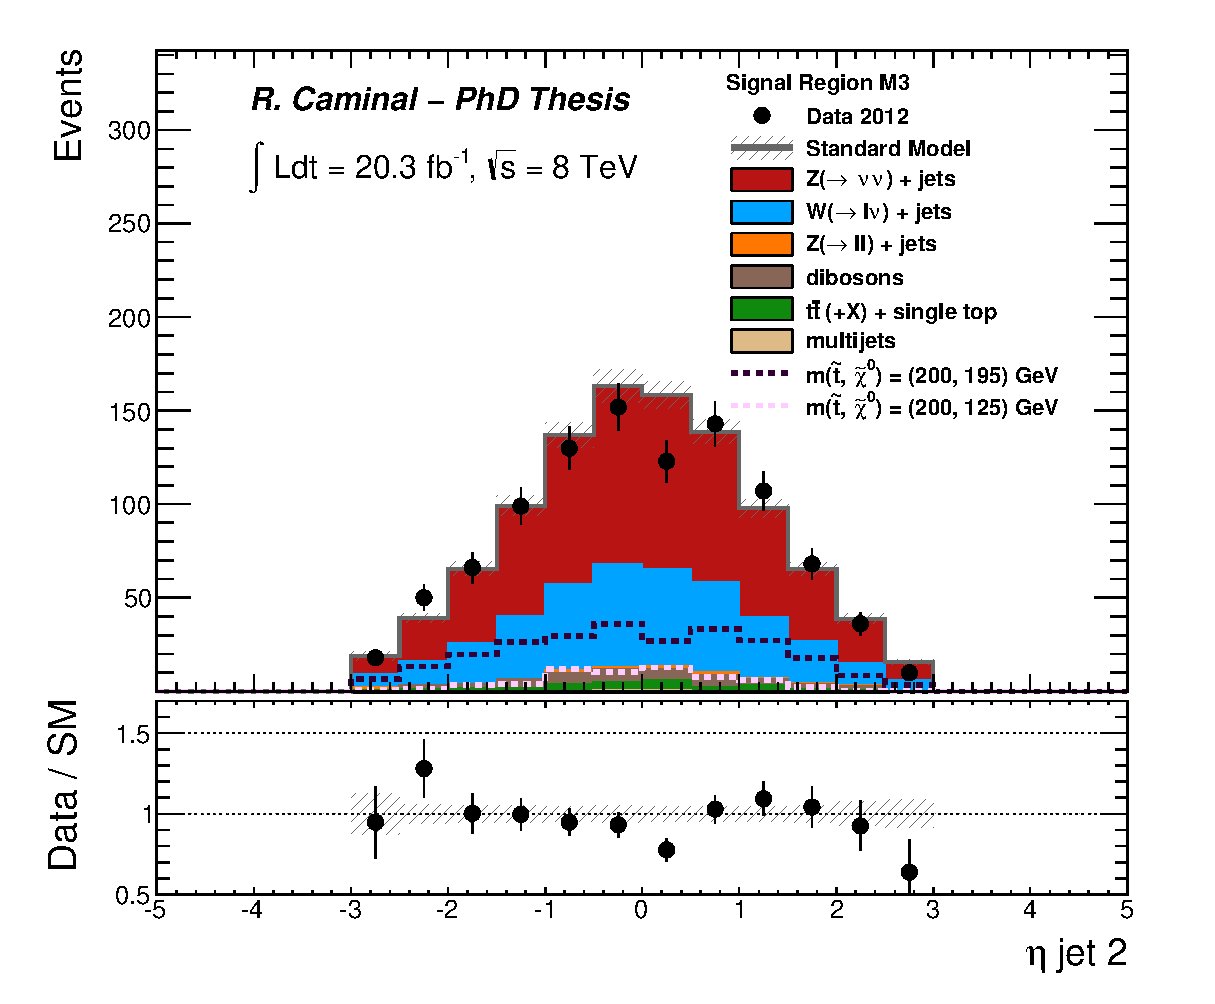
\includegraphics[width=0.495\textwidth]{MonojetAnalysis/Figures/plot_Stop_A4_SR_eta2_fitted.eps}
      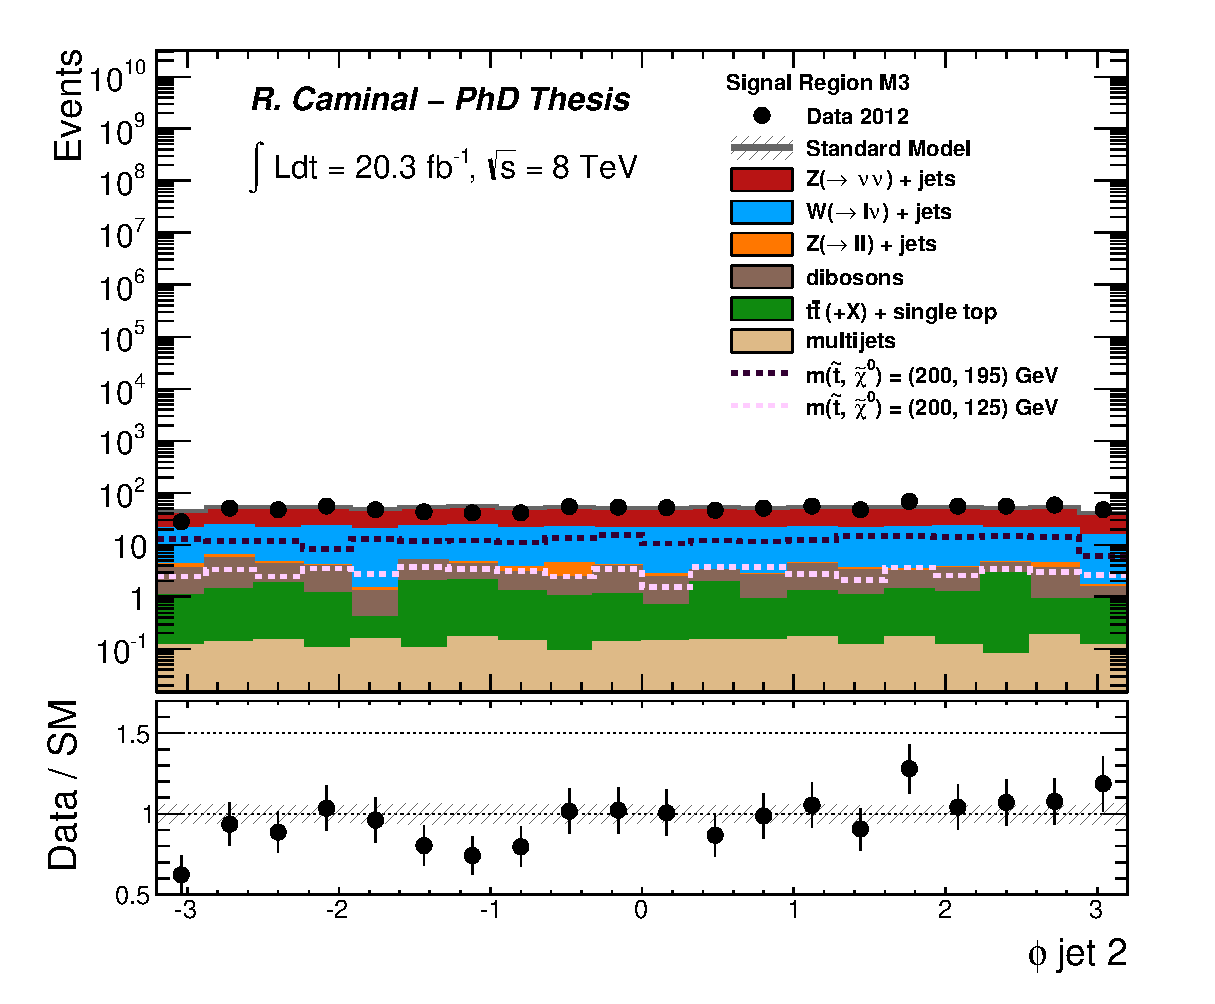
\includegraphics[width=0.495\textwidth]{MonojetAnalysis/Figures/plot_Stop_A4_SR_phi2_fitted.eps}
    }
  \end{center}
  \caption[Kinematic distributions of the $\pt$ of the second leading jet, the jet multiplicity, and the pseudo-rapidity and azimutal angle of the second leading jet in the signal regions for the selection cuts of region M3, after the normalization factors extracted from the fit have been applied.]
{The measured $\pt$ of the second leading jet (top left), the jet multiplicity (top right), and the pseudo-rapidity (bottom left) and azimutal angle (bottom right) of the second leading jet in the signal regions for the selection cuts of region M3, compared to the background predictions. The latter include the global normalization factors extracted from the fit. The error bands in the ratios include the statistical and experimental uncertainties on the background predictions. For illustration purposes, the distribution of two different SUSY scenarios for stop pair production are included.}
  \label{fig:Plot_M3_SR_Jet2}
\end{figure}

\begin{figure}[!ht]
  \begin{center}
    \mbox{
      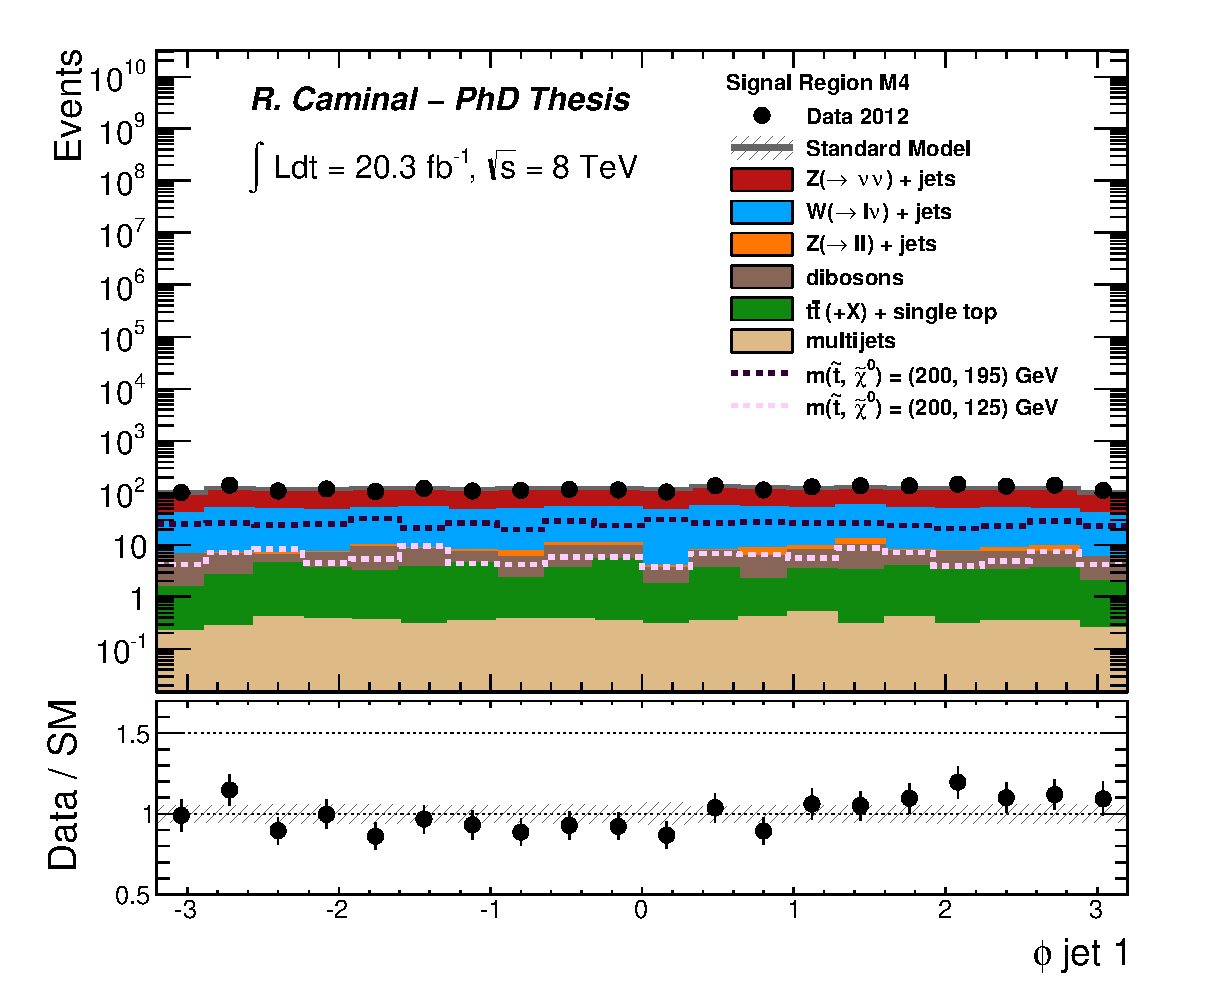
\includegraphics[width=0.495\textwidth]{MonojetAnalysis/Figures/plot_Stop_A8_SR_phi1_fitted.eps}
      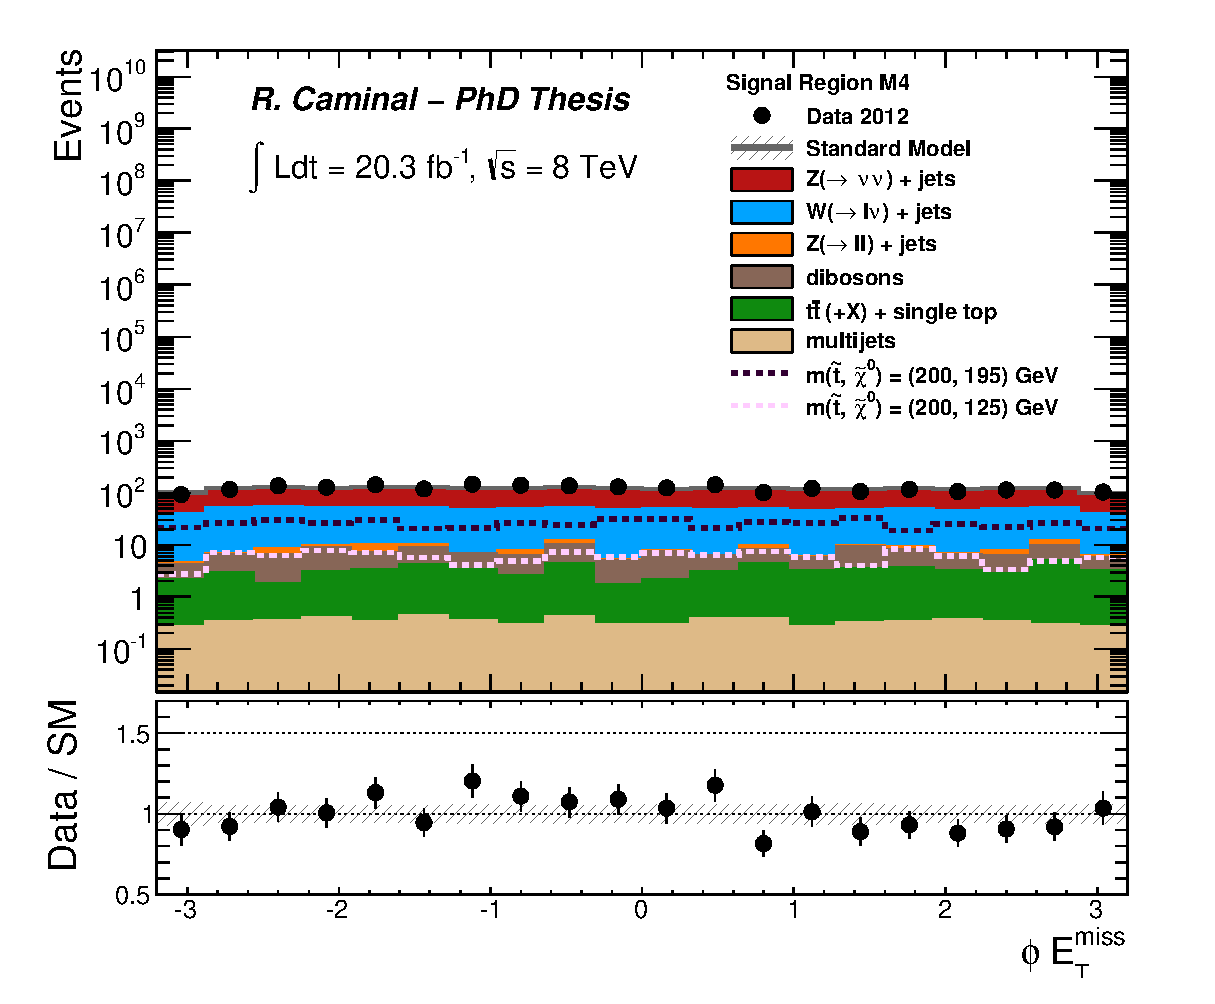
\includegraphics[width=0.495\textwidth]{MonojetAnalysis/Figures/plot_Stop_A8_SR_met_phi_fitted.eps}
    }
    \mbox{
      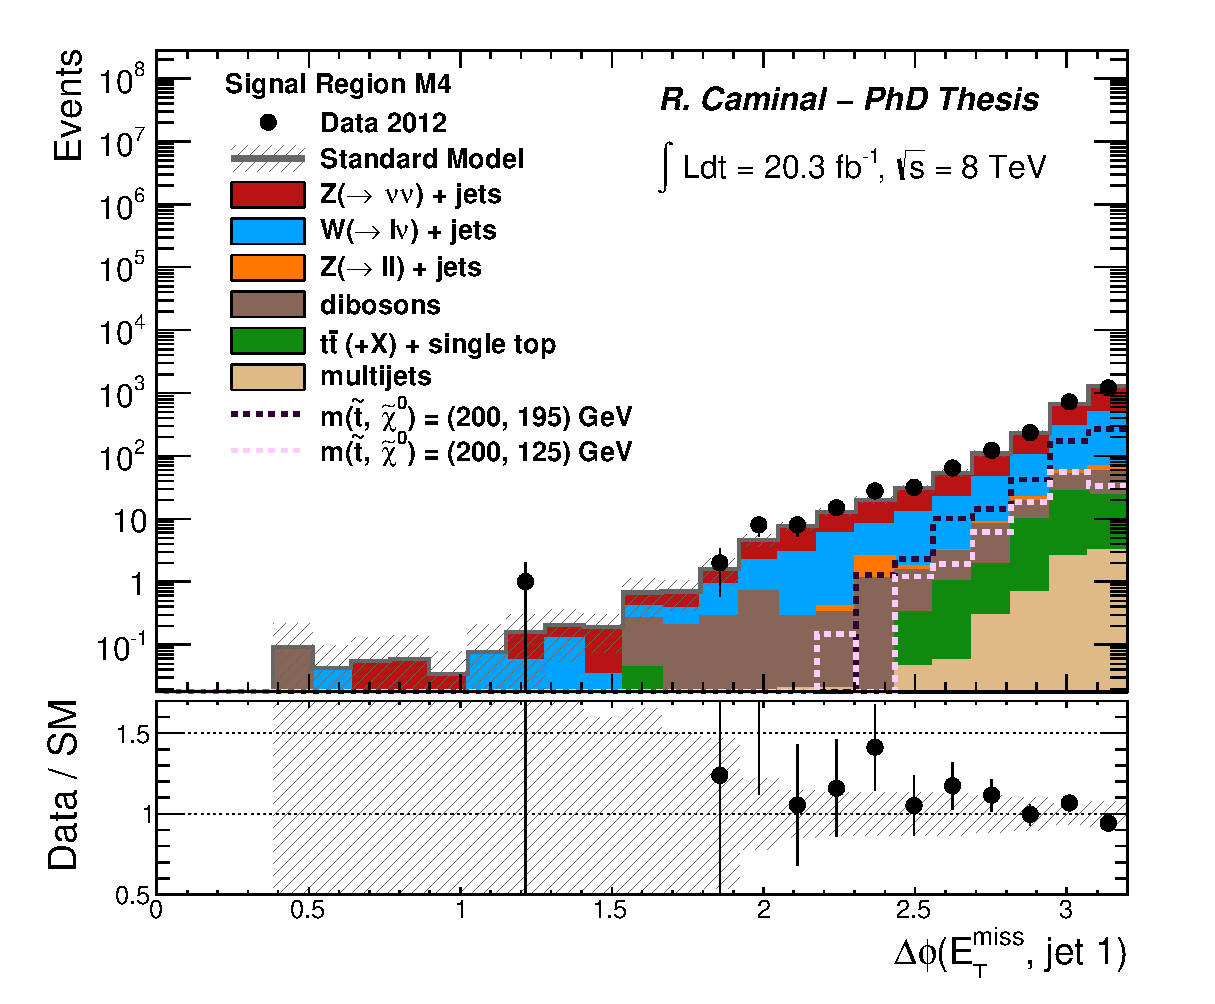
\includegraphics[width=0.495\textwidth]{MonojetAnalysis/Figures/plot_Stop_A8_SR_dPhi_met_j1_fitted.eps}
      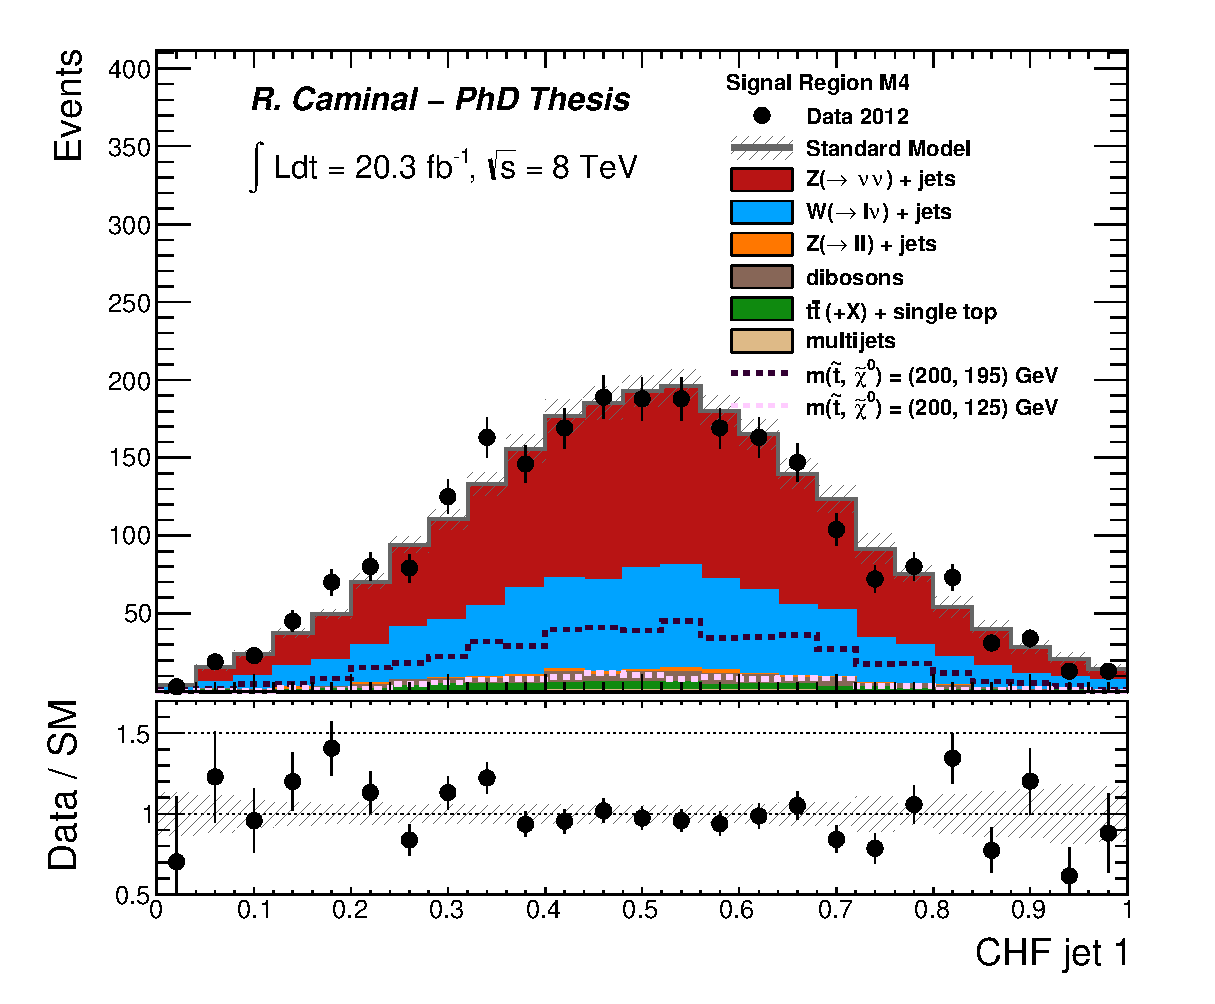
\includegraphics[width=0.495\textwidth]{MonojetAnalysis/Figures/plot_Stop_A8_SR_j1_chf_fitted.eps}
    }
    \mbox{
    }
  \end{center}
  \caption[Kinematic distributions of the azimutal angle, $\phi$, of the leading jet and the missing transverse energy, the azimutal angle difference between the leading jet and the $\met$, and the charge fraction of the leading jet in the signal regions for the selection cuts of region M4, after the normalization factors extracted from the fit have been applied.]
{The measured azimutal angle, $\phi$, of the leading jet (top left) and the missing transverse energy (top right), the azimutal angle difference between the leading jet and the $\met$ (bottom left) and the charge fraction of the leading jet (bottom right) for the selection cuts M4, compared to the background predictions. The latter include the global normalization factors extracted from the fit. The error bands in the ratios include the statistical and experimental uncertainties on the background predictions. For illustration purposes, the distribution of two different SUSY scenarios for stop pair production are included.}
  \label{fig:Plot_M4_SR_Jet1}
\end{figure}

\begin{figure}[!ht]
  \begin{center}
    \mbox{
      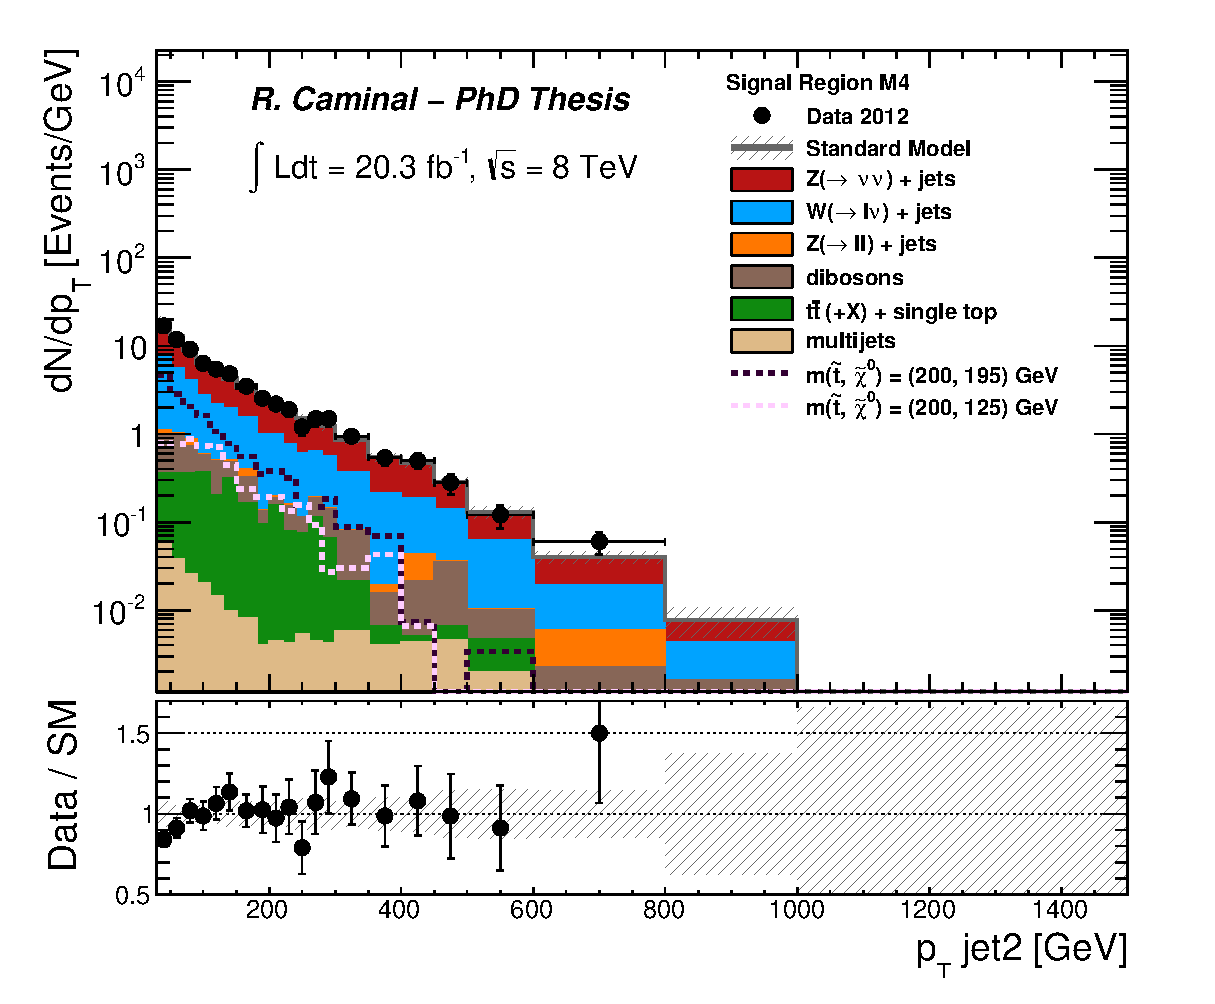
\includegraphics[width=0.495\textwidth]{MonojetAnalysis/Figures/plot_Stop_A8_SR_pt2_fitted.eps}
      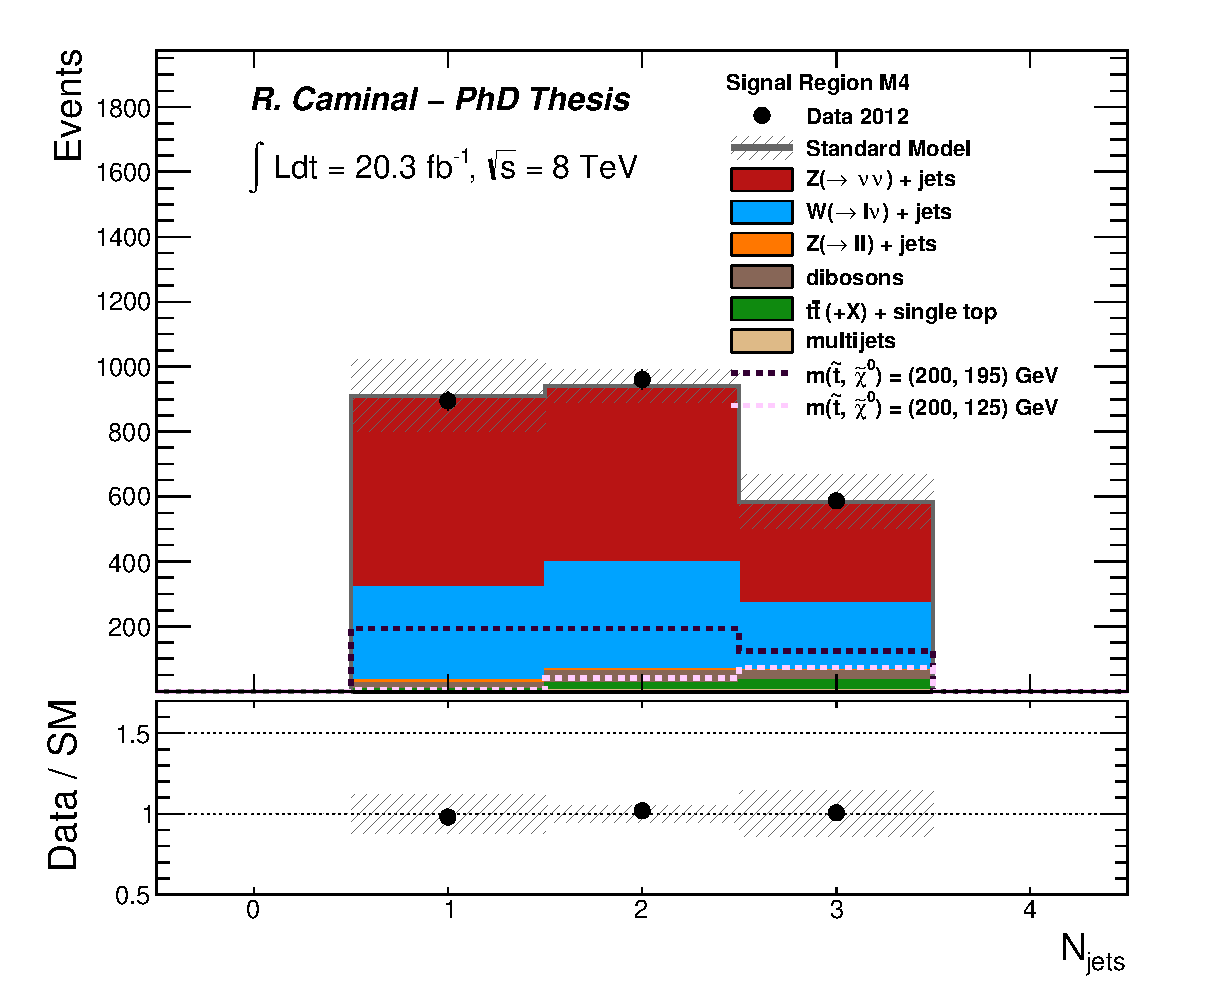
\includegraphics[width=0.495\textwidth]{MonojetAnalysis/Figures/plot_Stop_A8_SR_n_jets_fitted.eps}
    }
    \mbox{
      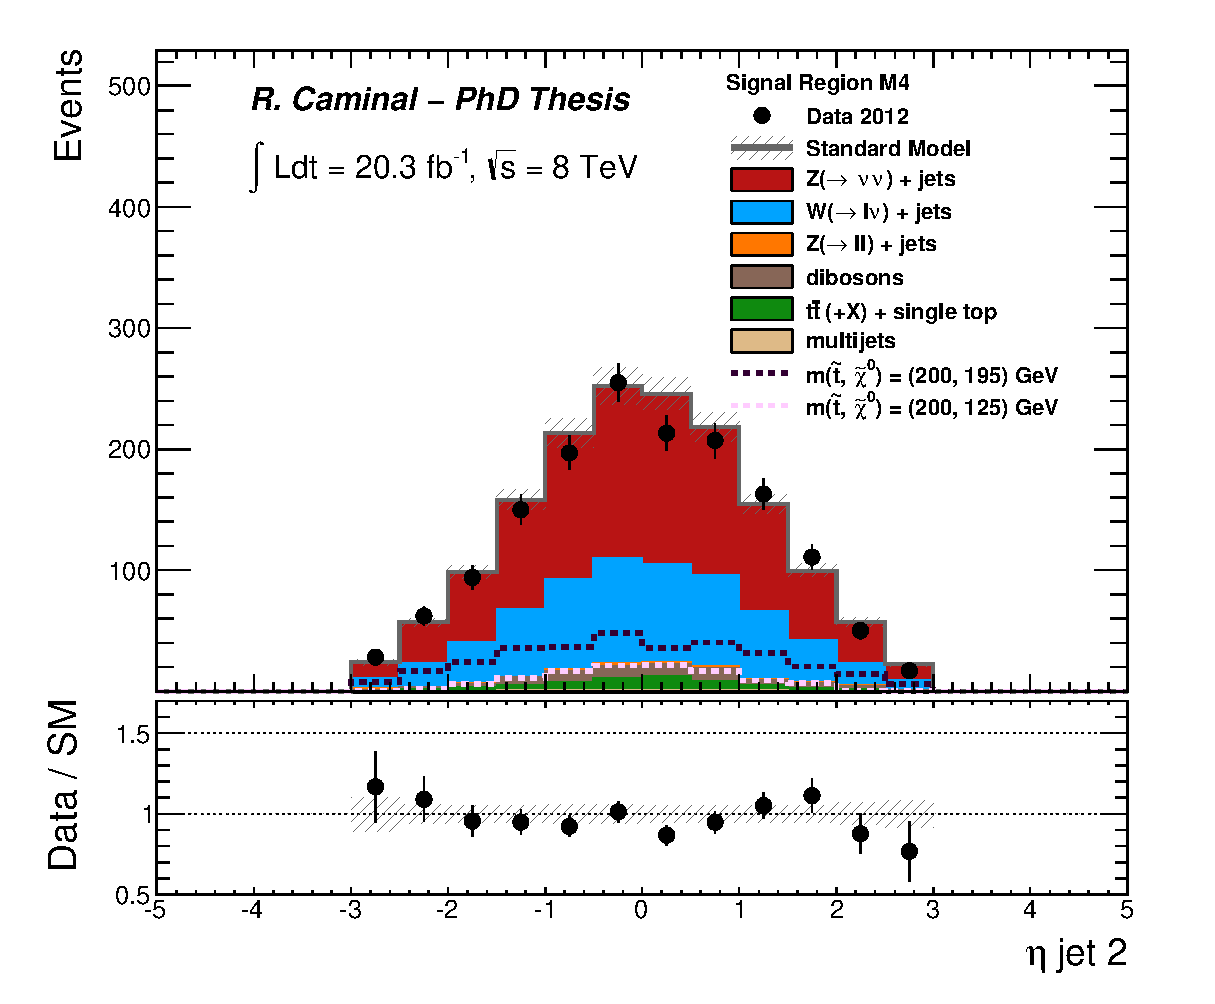
\includegraphics[width=0.495\textwidth]{MonojetAnalysis/Figures/plot_Stop_A8_SR_eta2_fitted.eps}
      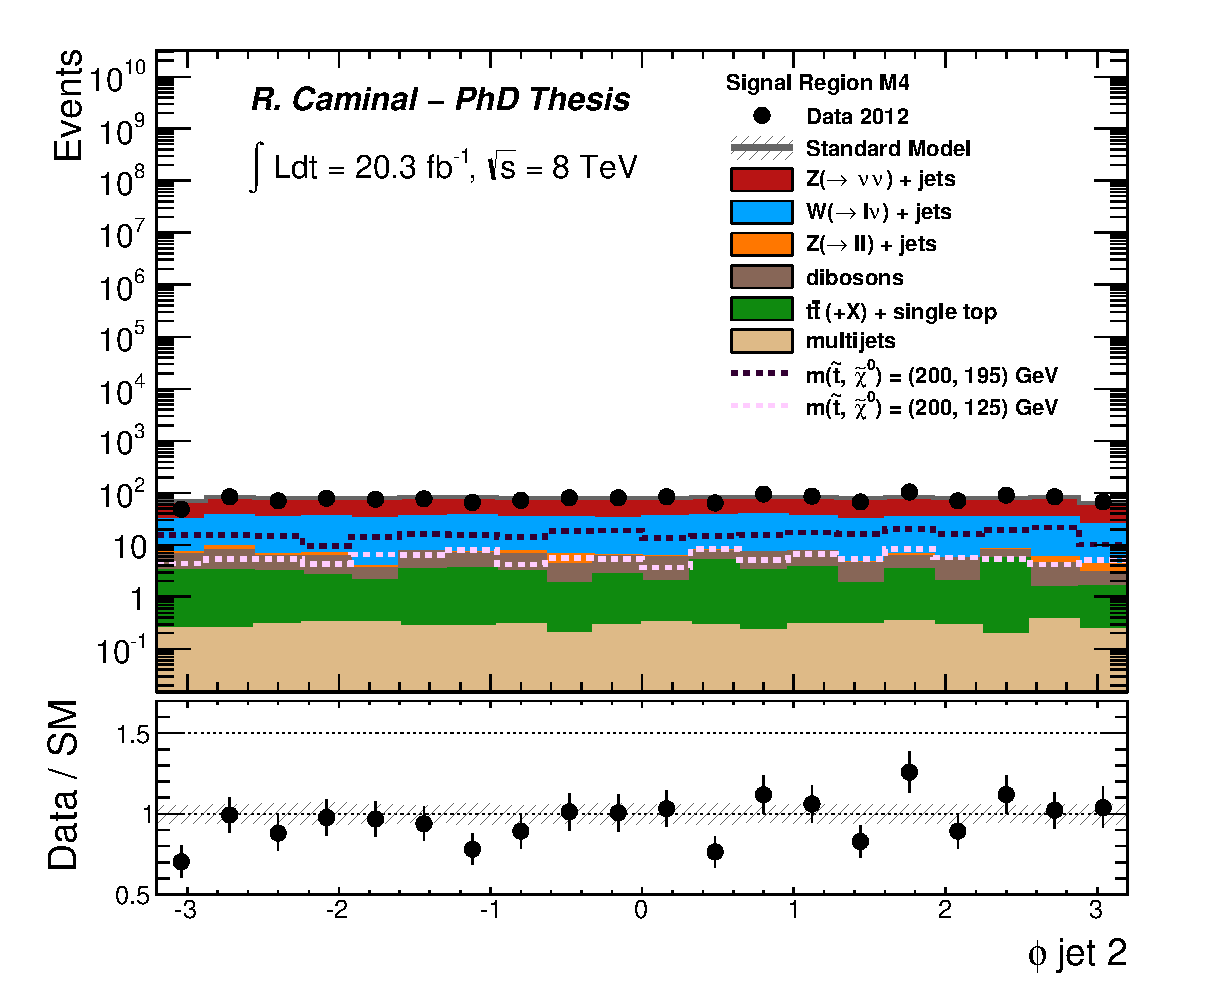
\includegraphics[width=0.495\textwidth]{MonojetAnalysis/Figures/plot_Stop_A8_SR_phi2_fitted.eps}
    }
  \end{center}
  \caption[Kinematic distributions of the $\pt$ of the second leading jet, the jet multiplicity, and the pseudo-rapidity and azimutal angle of the second leading jet in the signal regions for the selection cuts of region M4, after the normalization factors extracted from the fit have been applied.]
{The measured $\pt$ of the second leading jet (top left), the jet multiplicity (top right), and the pseudo-rapidity (bottom left) and azimutal angle (bottom right) of the second leading jet in the signal regions for the selection cuts of region M4, compared to the background predictions. The latter include the global normalization factors extracted from the fit. The error bands in the ratios include the statistical and experimental uncertainties on the background predictions. For illustration purposes, the distribution of two different SUSY scenarios for stop pair production are included.}
  \label{fig:Plot_M4_SR_Jet2}
\end{figure}

\begin{figure}[!ht]
  \begin{center}
    \mbox{
      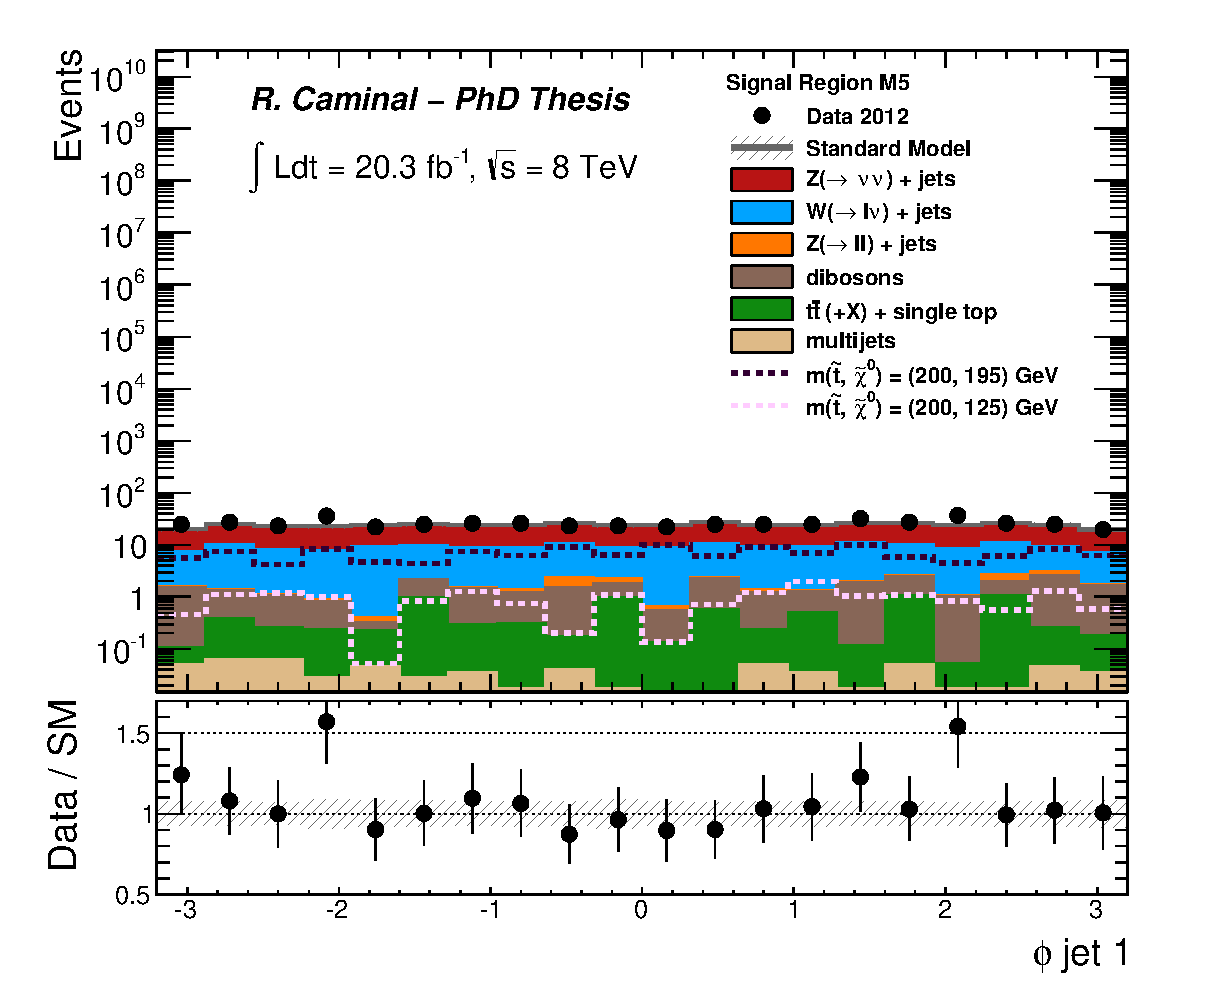
\includegraphics[width=0.495\textwidth]{MonojetAnalysis/Figures/plot_Stop_A9_SR_phi1_fitted.eps}
      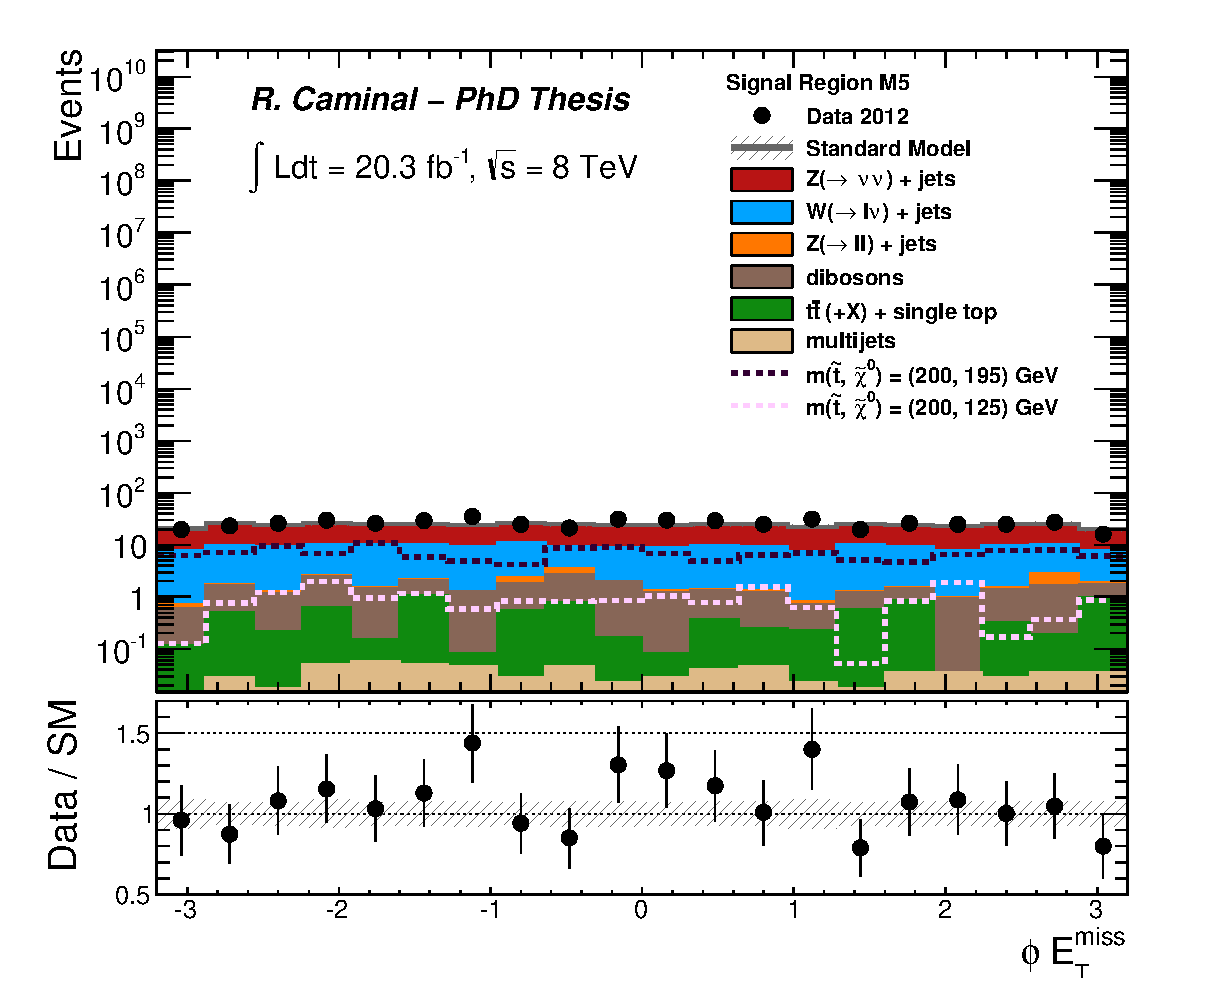
\includegraphics[width=0.495\textwidth]{MonojetAnalysis/Figures/plot_Stop_A9_SR_met_phi_fitted.eps}
    }
    \mbox{
      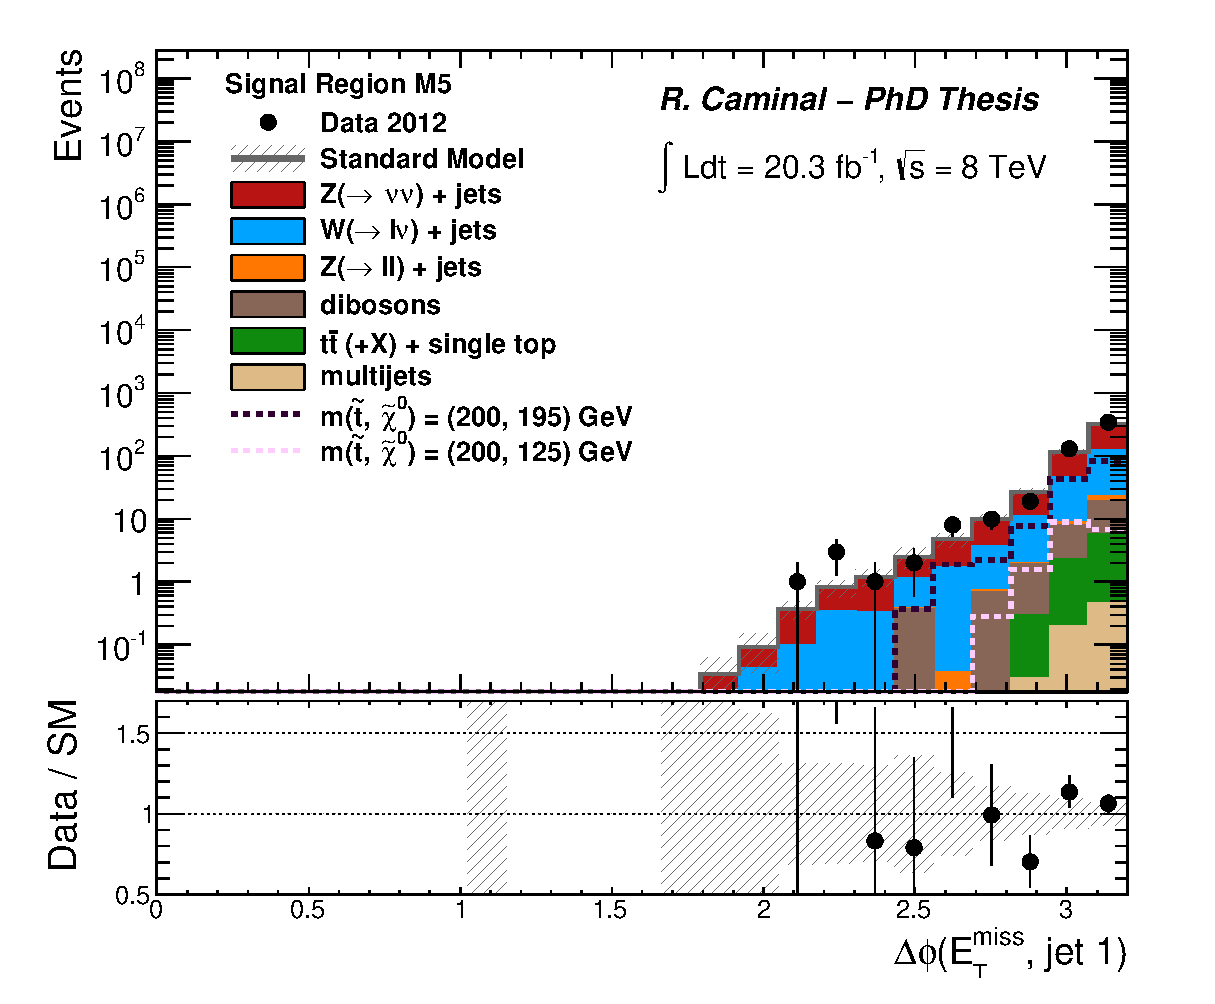
\includegraphics[width=0.495\textwidth]{MonojetAnalysis/Figures/plot_Stop_A9_SR_dPhi_met_j1_fitted.eps}
      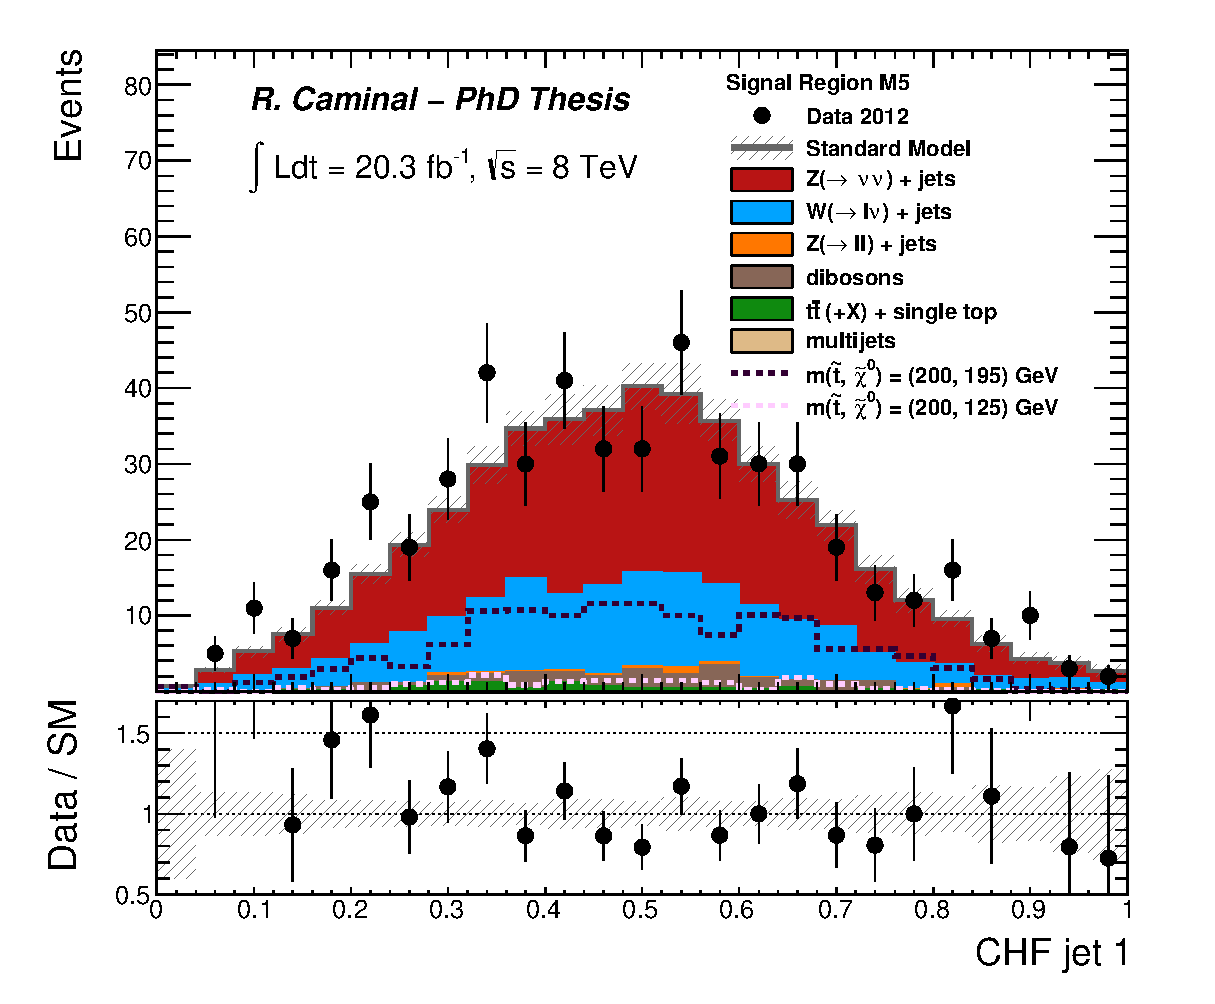
\includegraphics[width=0.495\textwidth]{MonojetAnalysis/Figures/plot_Stop_A9_SR_j1_chf_fitted.eps}
    }
  \end{center}
  \caption[Kinematic distributions of the azimutal angle, $\phi$, of the leading jet and the missing transverse energy, the azimutal angle difference between the leading jet and the $\met$, and the charge fraction of the leading jet in the signal regions for the selection cuts of region M5, after the normalization factors extracted from the fit have been applied.]
{The measured azimutal angle, $\phi$, of the leading jet (top left) and the missing transverse energy (top right), the azimutal angle difference between the leading jet and the $\met$ (bottom left) and the charge fraction of the leading jet (bottom right) for the selection cuts M5, compared to the background predictions. The latter include the global normalization factors extracted from the fit. The error bands in the ratios include the statistical and experimental uncertainties on the background predictions. For illustration purposes, the distribution of two different SUSY scenarios for stop pair production are included.}
  \label{fig:Plot_M5_SR_Jet1}
\end{figure}

\begin{figure}[!ht]
  \begin{center}
    \mbox{
      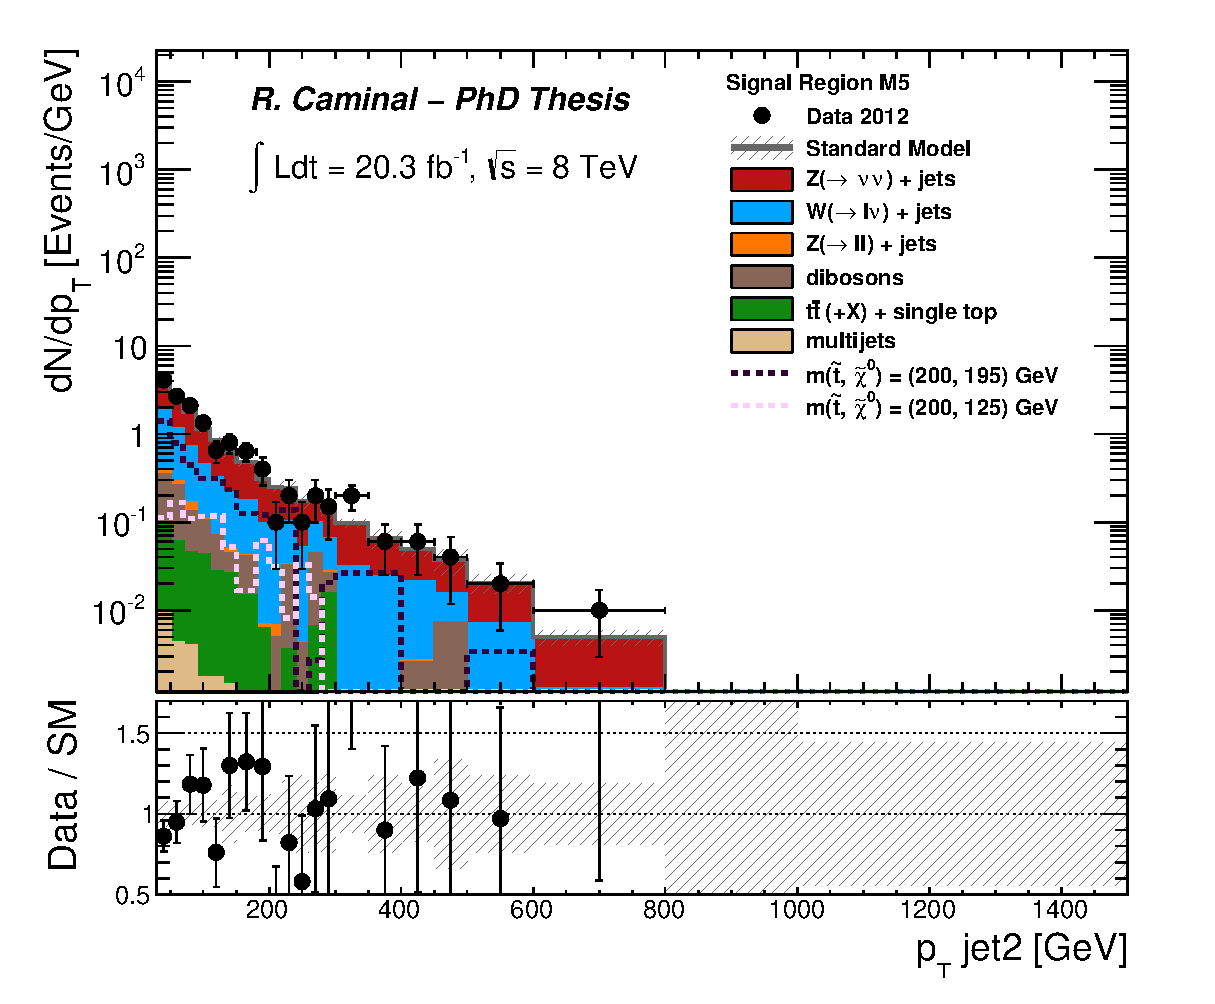
\includegraphics[width=0.495\textwidth]{MonojetAnalysis/Figures/plot_Stop_A9_SR_pt2_fitted.eps}
      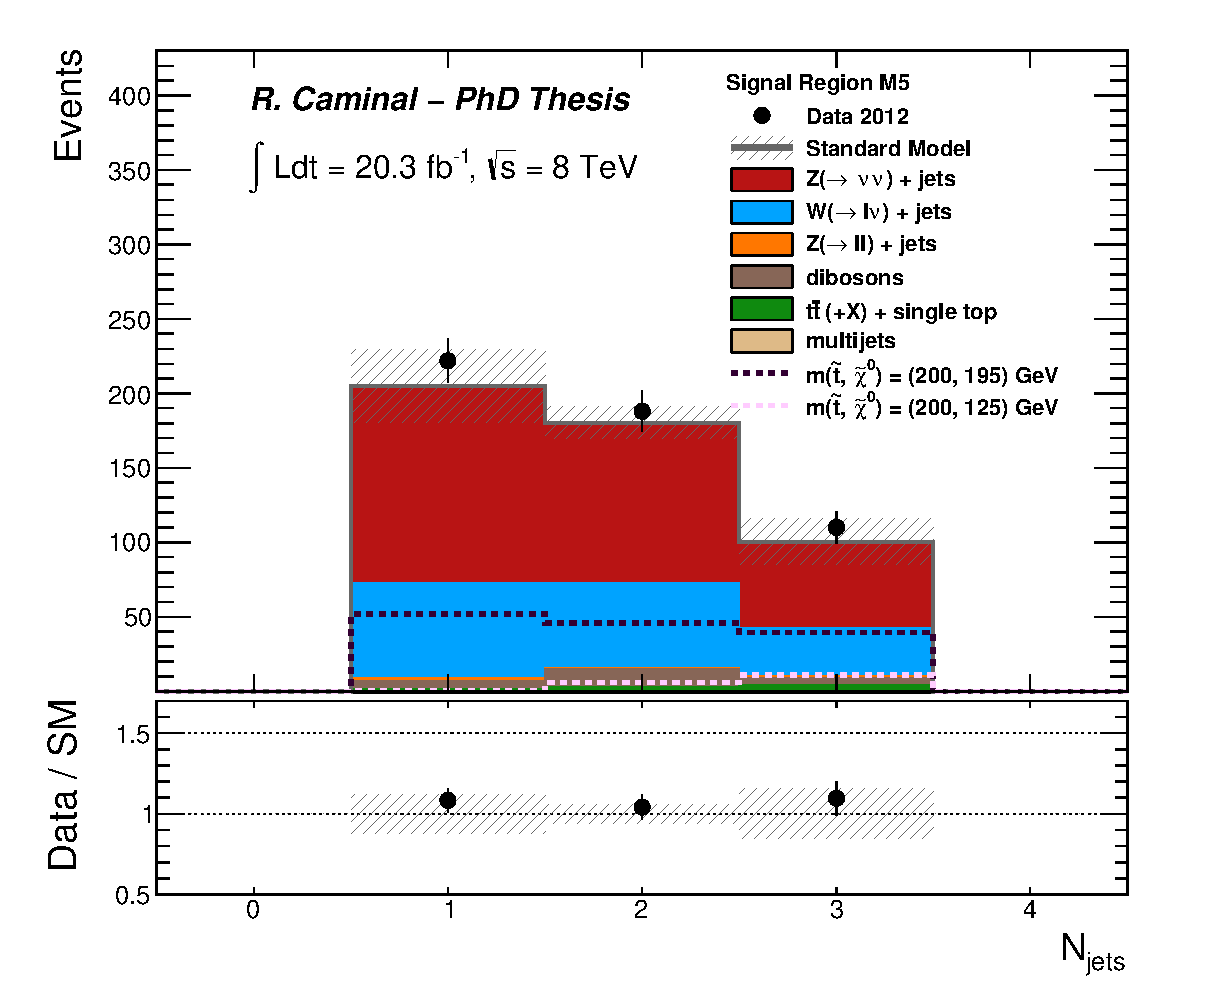
\includegraphics[width=0.495\textwidth]{MonojetAnalysis/Figures/plot_Stop_A9_SR_n_jets_fitted.eps}
    }
    \mbox{
      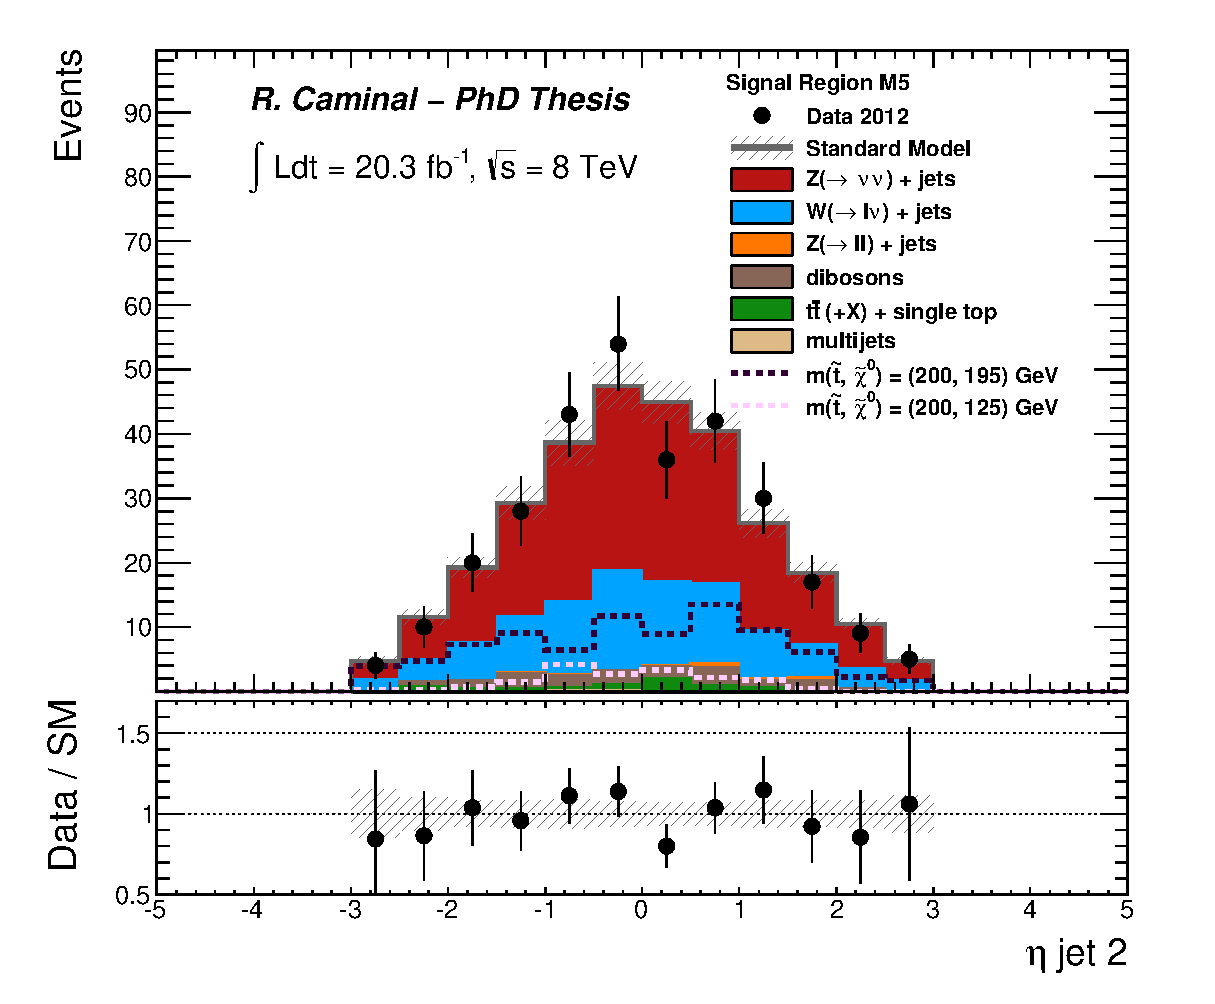
\includegraphics[width=0.495\textwidth]{MonojetAnalysis/Figures/plot_Stop_A9_SR_eta2_fitted.eps}
      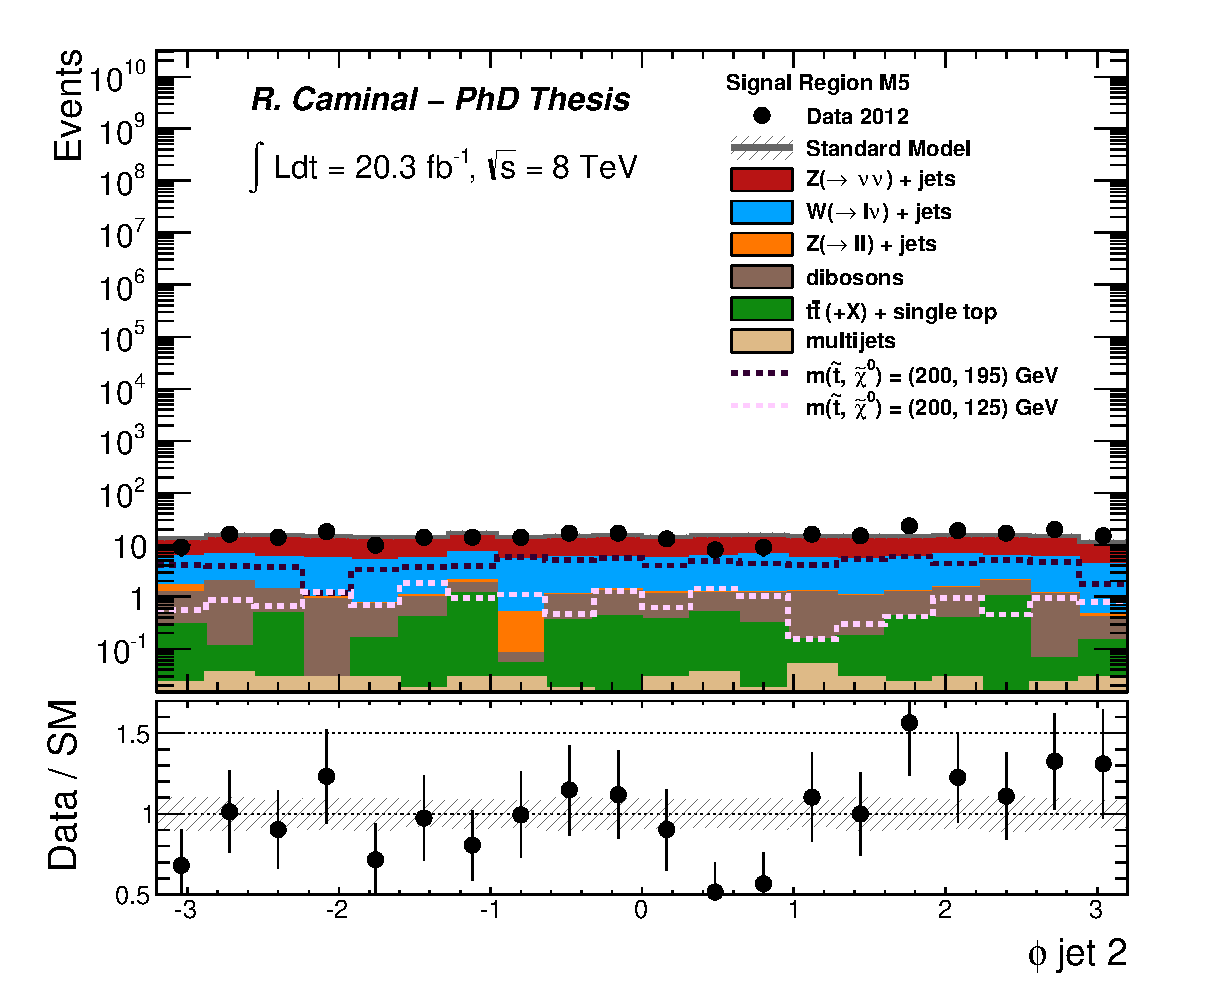
\includegraphics[width=0.495\textwidth]{MonojetAnalysis/Figures/plot_Stop_A9_SR_phi2_fitted.eps}
    }
  \end{center}
  \caption[Kinematic distributions of the $\pt$ of the second leading jet, the jet multiplicity, and the pseudo-rapidity and azimutal angle of the second leading jet in the signal regions for the selection cuts of region M5, after the normalization factors extracted from the fit have been applied.]
{The measured $\pt$ of the second leading jet (top left), the jet multiplicity (top right), and the pseudo-rapidity (bottom left) and azimutal angle (bottom right) of the second leading jet in the signal regions for the selection cuts of region M5, compared to the background predictions. The latter include the global normalization factors extracted from the fit. The error bands in the ratios include the statistical and experimental uncertainties on the background predictions. For illustration purposes, the distribution of two different SUSY scenarios for stop pair production are included.}
  \label{fig:Plot_M5_SR_Jet2}
\end{figure}

\begin{figure}[!ht]
  \begin{center}
    \mbox{
      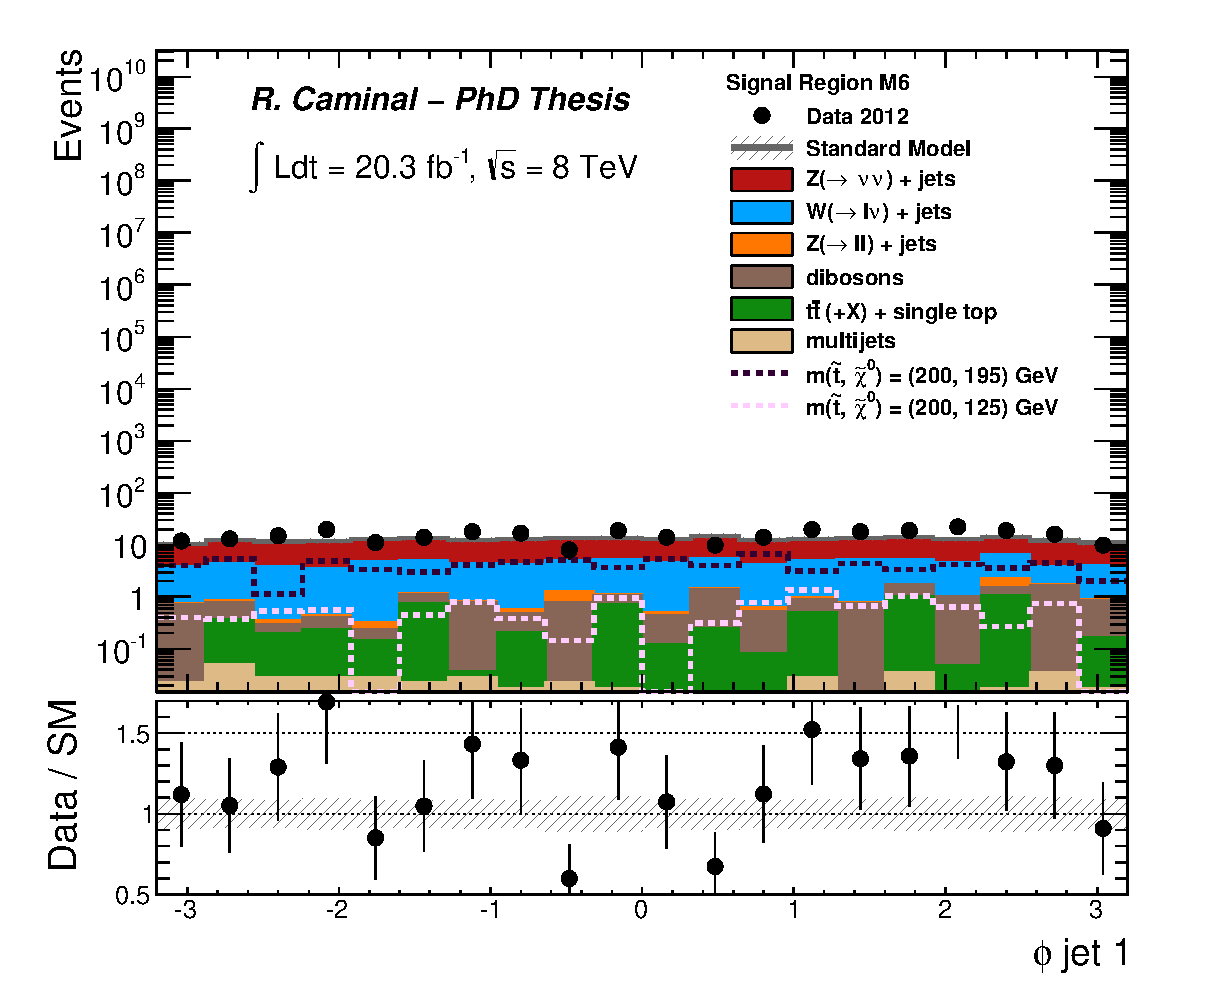
\includegraphics[width=0.495\textwidth]{MonojetAnalysis/Figures/plot_Stop_A10_SR_phi1_fitted.eps}
      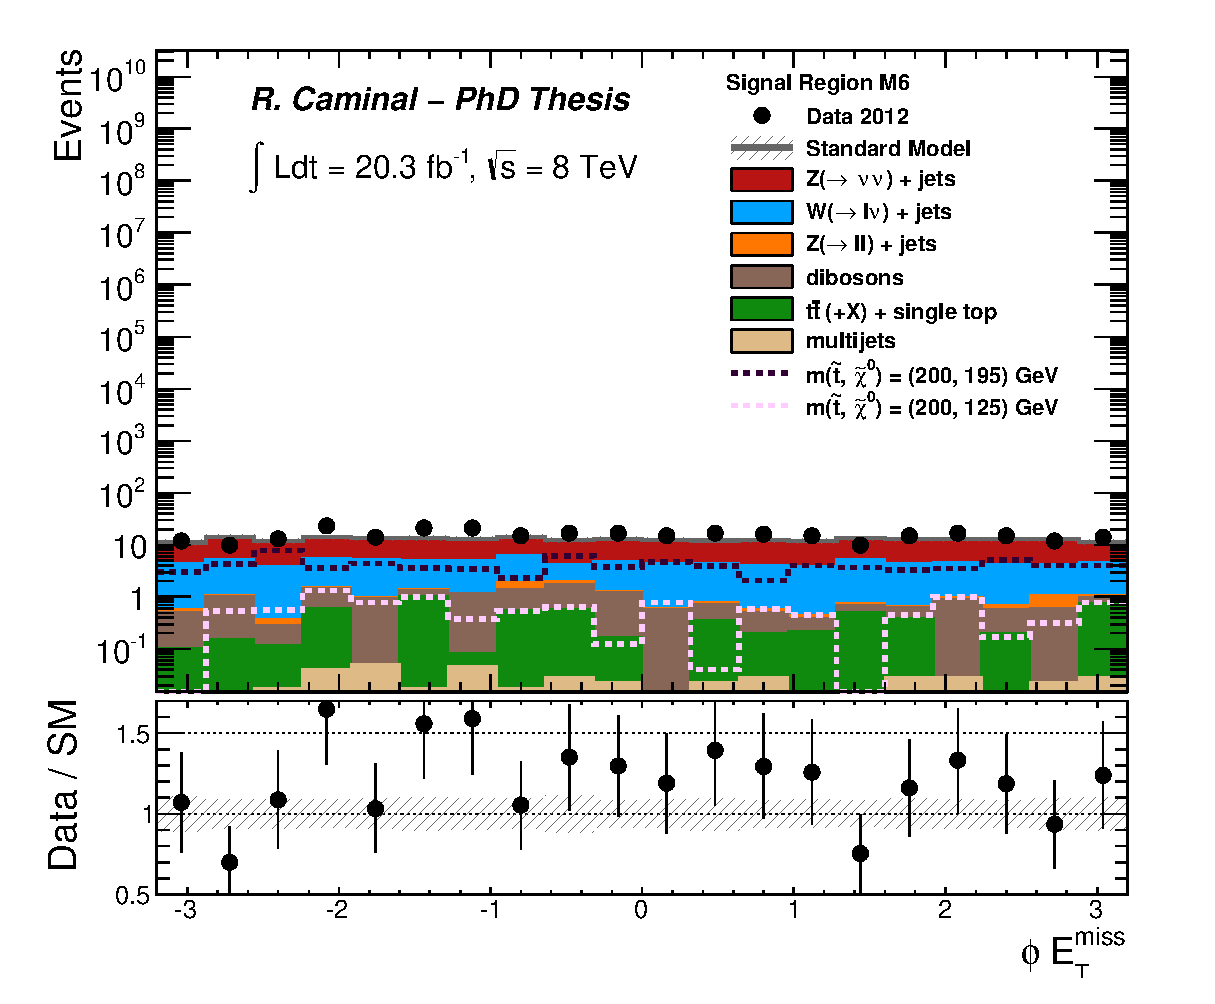
\includegraphics[width=0.495\textwidth]{MonojetAnalysis/Figures/plot_Stop_A10_SR_met_phi_fitted.eps}
    }
    \mbox{
      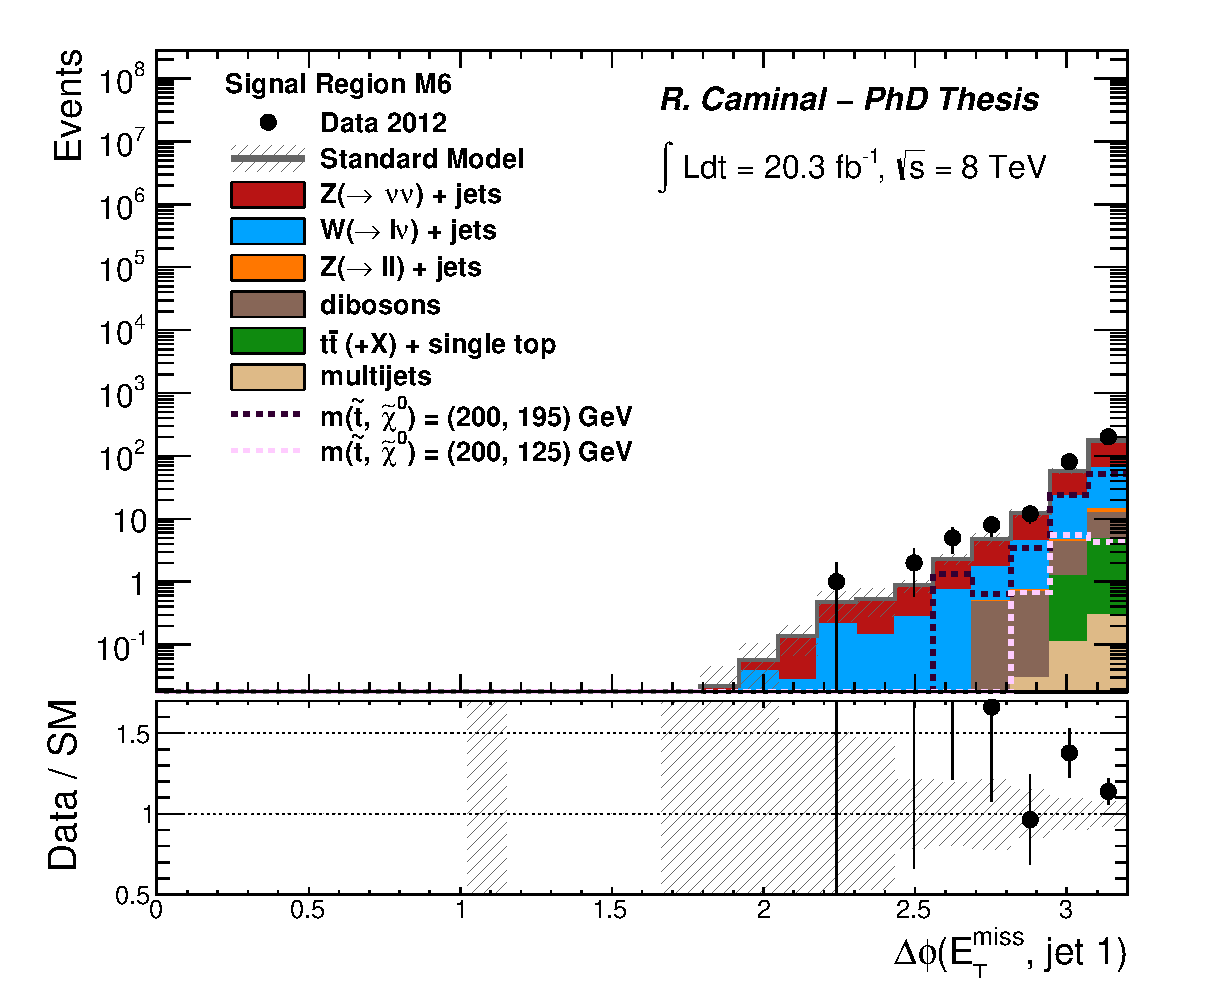
\includegraphics[width=0.495\textwidth]{MonojetAnalysis/Figures/plot_Stop_A10_SR_dPhi_met_j1_fitted.eps}
      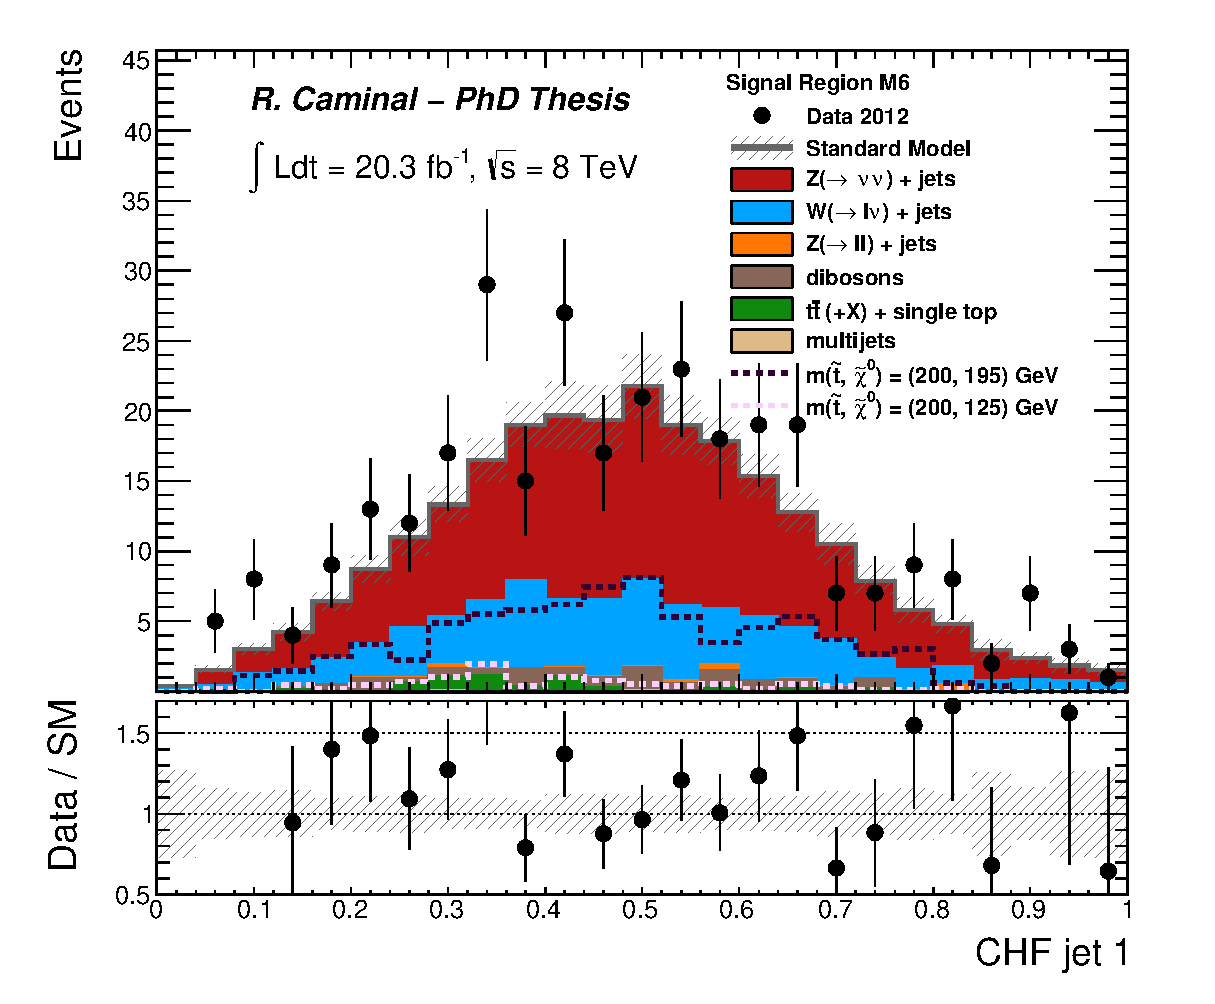
\includegraphics[width=0.495\textwidth]{MonojetAnalysis/Figures/plot_Stop_A10_SR_j1_chf_fitted.eps}
    }
  \end{center}
  \caption[Kinematic distributions of the azimutal angle, $\phi$, of the leading jet and the missing transverse energy, the azimutal angle difference between the leading jet and the $\met$, and the charge fraction of the leading jet in the signal regions for the selection cuts of region M6, after the normalization factors extracted from the fit have been applied.]
{The measured azimutal angle, $\phi$, of the leading jet (top left) and the missing transverse energy (top right), the azimutal angle difference between the leading jet and the $\met$ (bottom left) and the charge fraction of the leading jet (bottom right) for the selection cuts M6, compared to the background predictions. The latter include the global normalization factors extracted from the fit. The error bands in the ratios include the statistical and experimental uncertainties on the background predictions. For illustration purposes, the distribution of two different SUSY scenarios for stop pair production are included.}
  \label{fig:Plot_M6_SR_Jet1}
\end{figure}

\begin{figure}[!ht]
  \begin{center}
    \mbox{
      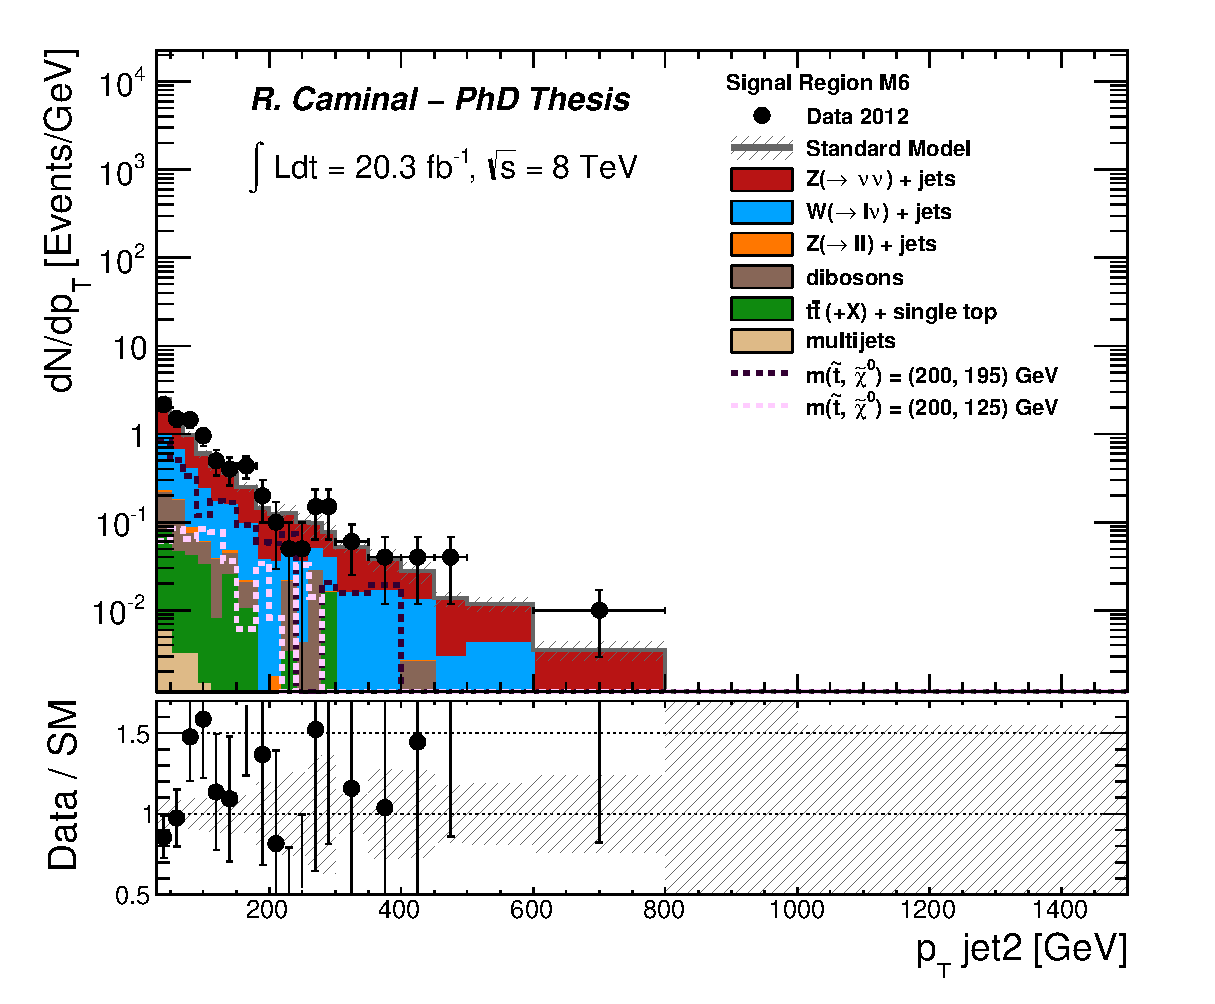
\includegraphics[width=0.495\textwidth]{MonojetAnalysis/Figures/plot_Stop_A10_SR_pt2_fitted.eps}
      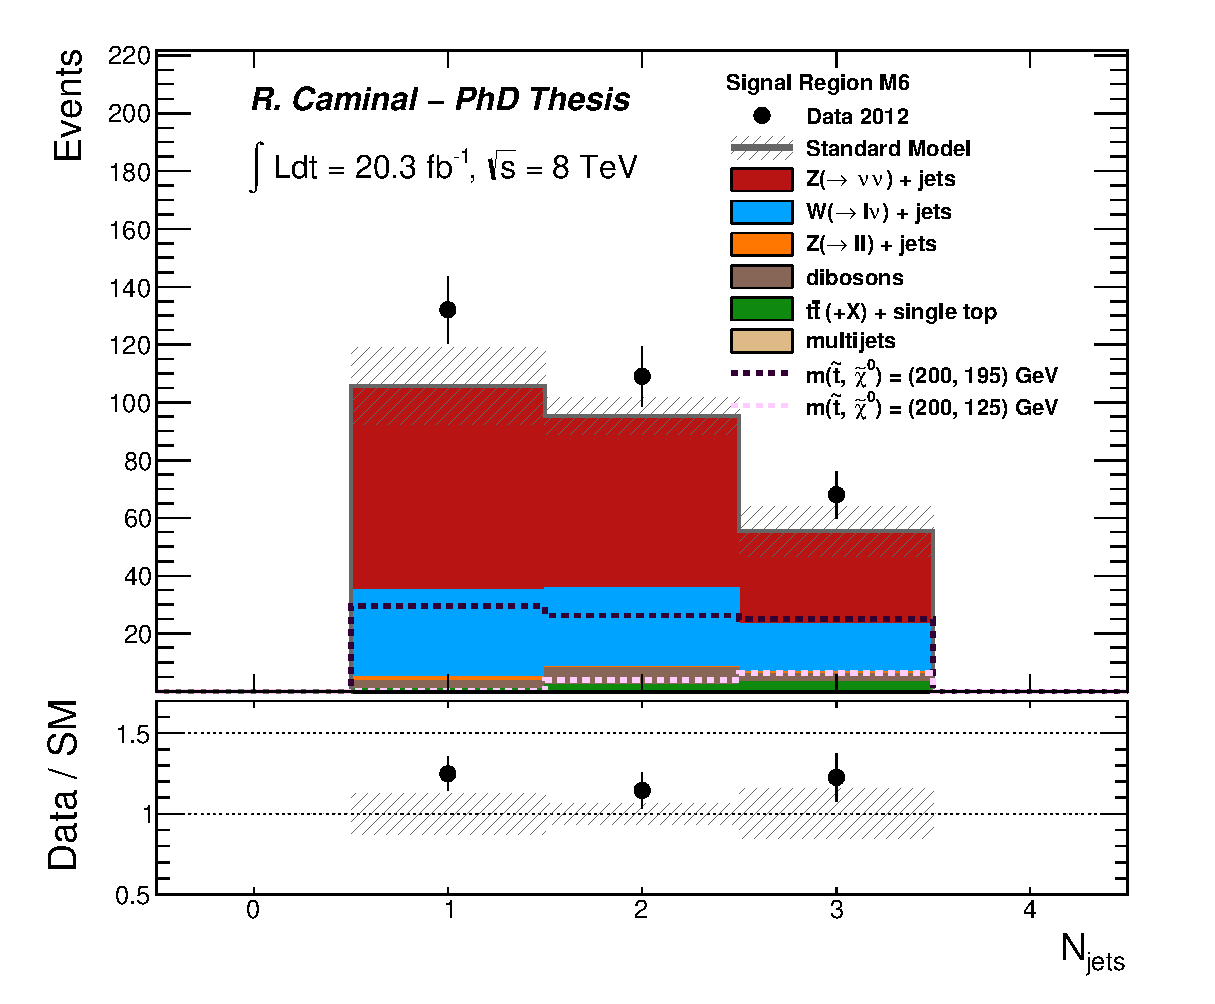
\includegraphics[width=0.495\textwidth]{MonojetAnalysis/Figures/plot_Stop_A10_SR_n_jets_fitted.eps}
    }
    \mbox{
      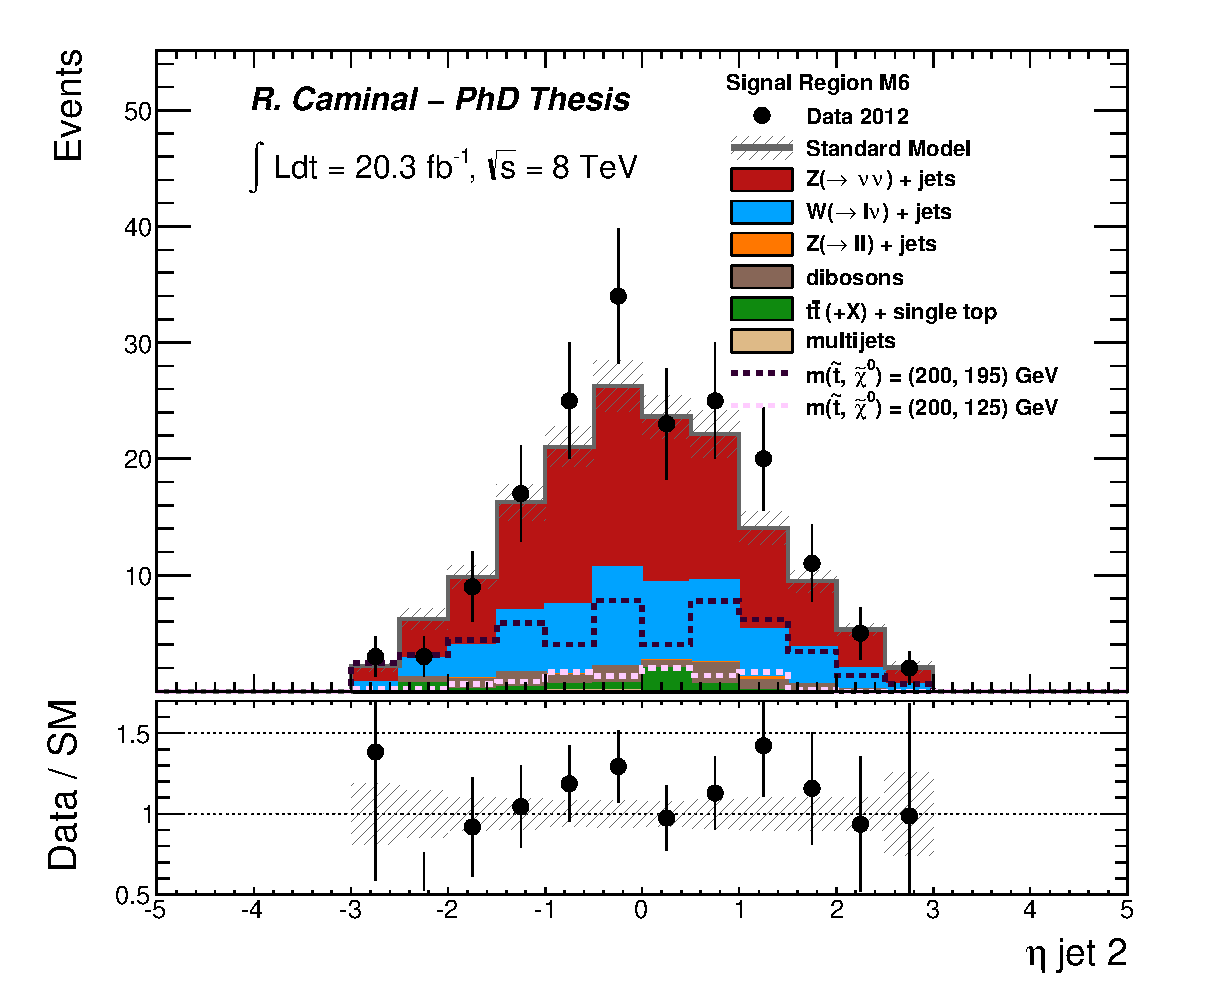
\includegraphics[width=0.495\textwidth]{MonojetAnalysis/Figures/plot_Stop_A10_SR_eta2_fitted.eps}
      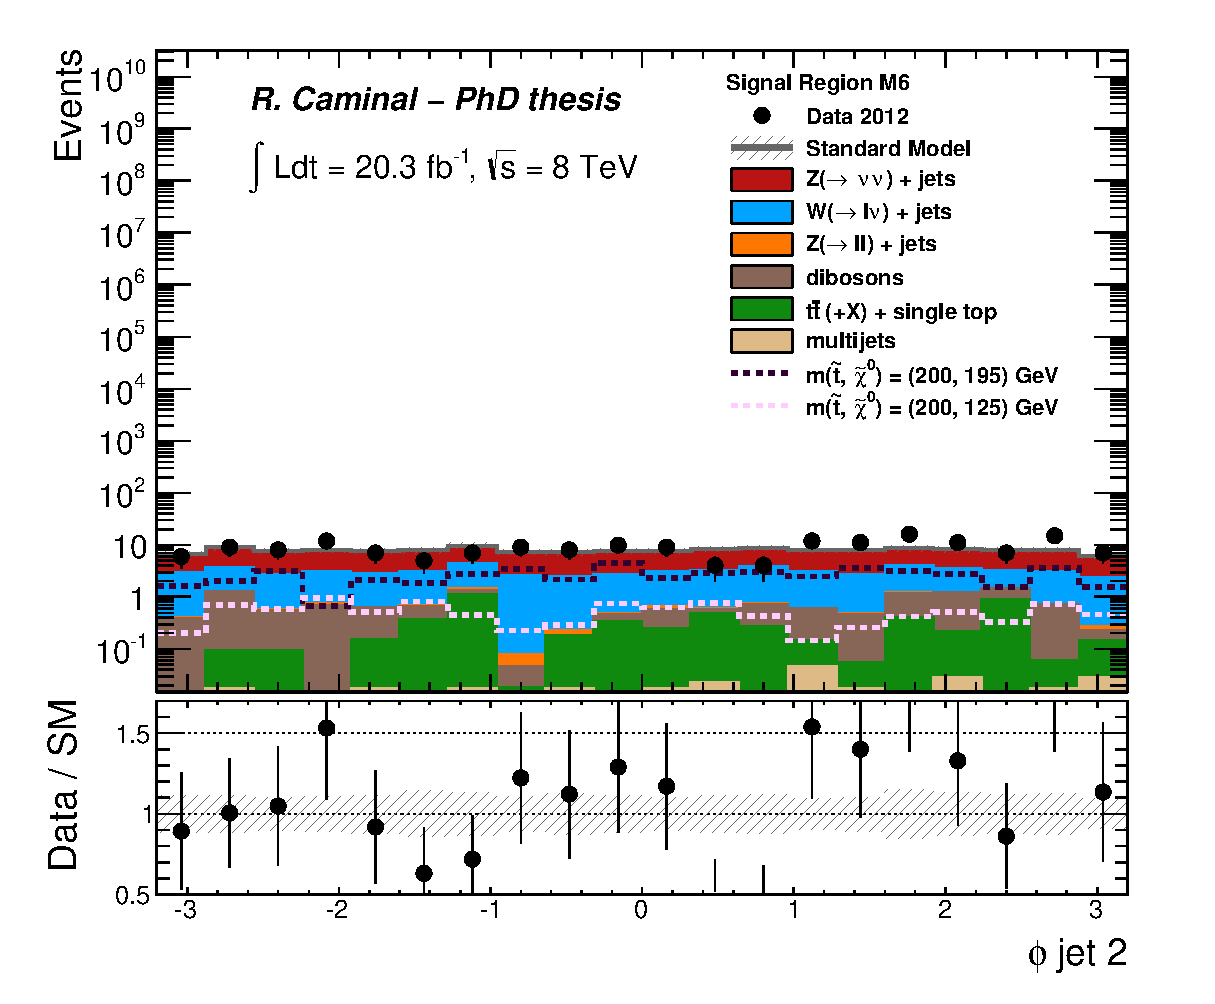
\includegraphics[width=0.495\textwidth]{MonojetAnalysis/Figures/plot_Stop_A10_SR_phi2_fitted.eps}
    }
  \end{center}
  \caption[Kinematic distributions of the $\pt$ of the second leading jet, the jet multiplicity, and the pseudo-rapidity and azimutal angle of the second leading jet in the signal regions for the selection cuts of region M6, after the normalization factors extracted from the fit have been applied.]
{The measured $\pt$ of the second leading jet (top left), the jet multiplicity (top right), and the pseudo-rapidity (bottom left) and azimutal angle (bottom right) of the second leading jet in the signal regions for the selection cuts of region M6, compared to the background predictions. The latter include the global normalization factors extracted from the fit. The error bands in the ratios include the statistical and experimental uncertainties on the background predictions. For illustration purposes, the distribution of two different SUSY scenarios for stop pair production are included.}
  \label{fig:Plot_M6_SR_Jet2}
\end{figure}

